\documentclass[final,1p,11pt,longtitle]{elsarticle}

\usepackage{amsmath}
\usepackage{amssymb}
\usepackage{graphicx}
\usepackage{hyperref}
\usepackage{multirow}


% Bilingual reading copy: display equations are shared, verbatim from main.tex.
\usepackage{fontspec}
\setmainfont{NotoSerif-Regular.ttf}[
 Path=fonts/,
 BoldFont=NotoSerif-Bold.ttf,
 ItalicFont=NotoSerif-Italic.ttf,
 BoldItalicFont=NotoSerif-BoldItalic.ttf]
\usepackage{xcolor}
\definecolor{viColor}{HTML}{17606A}
\geometry{reset,a4paper,margin=22mm}
\setlength{\emergencystretch}{3em}
\newenvironment{viet}{\par\smallskip\begingroup\color{viColor}\noindent\textbf{VI. }\ignorespaces}{\par\endgroup\smallskip}
\newcommand{\tablevi}[2]{\shortstack[l]{#1\\{\color{viColor}\scriptsize #2}}}
\abstracttitle{Abstract / Tóm tắt}
\keywordtitle{Keywords / Từ khóa}
\renewcommand{\figurename}{Figure / Hình}
\renewcommand{\tablename}{Table / Bảng}
\renewcommand{\refname}{References / Tài liệu tham khảo}
\hypersetup{unicode=true,colorlinks=true,linkcolor=viColor,citecolor=viColor,urlcolor=viColor}

\journal{Smart Agricultural Technology}

\begin{document}

\begin{frontmatter}

\title{Automated Phenotypic Trait Extraction from Longitudinally Sectioned Chili Pepper Fruits Using Instance Segmentation\\[0.6em]{\large\color{viColor} Tự động trích xuất đặc trưng kiểu hình từ quả ớt cắt dọc bằng phân đoạn thực thể}}
%%Anh Tuấn kêu điền dô nma chưa nghĩa ga :>
%% BỎ TRỐNG TOÀN BỘ PHẦN \author Ở ĐÂY (DOUBLE ANONYMIZED PEER REVIEW)

%% Tác giả 1
\author[1,2]{Thuy Nguyen Thi Nhu\fnref{fn1}}
\ead{24521755@uit.edu.vn}

%% Tác giả 2
\author[1,2]{Trong Tai Ha\fnref{fn1}}
\ead{21520436@uit.edu.vn}

\author[1,2]{Chau Anh Le\fnref{fn1}}
\ead{21511821@uit.edu.vn}

%% Tác giả 3
\author[1,2,3]{Thanh Tuan Thai}
\ead{tuantt@uit.edu.vn}

%% Tác giả 4
\author[1,2]{Tien Dung Mai}
\ead{dungmt@uit.edu.vn}

%% Tác giả 6 (Corresponding)
\author[3]{Yong Suk Chung\corref{cor1}}
\ead{yschung@jejunu.ac.kr}

%%%%%% Affiliations %%%%%%
\address[1]{Faculty of Computer Science, University of Information Technology, Ho Chi Minh city 70000, Vietnam\\{\color{viColor} Khoa Khoa học Máy tính, Trường Đại học Công nghệ Thông tin, Thành phố Hồ Chí Minh 70000, Việt Nam}}
\address[2]{Vietnam National University, Ho Chi Minh city 70000, Vietnam\\{\color{viColor} Đại học Quốc gia Thành phố Hồ Chí Minh, Thành phố Hồ Chí Minh 70000, Việt Nam}}
\address[3]{Department of Plant Resources and Environment, Jeju National University, Jeju 63243, Republic of Korea\\{\color{viColor} Khoa Tài nguyên Thực vật và Môi trường, Đại học Quốc gia Jeju, Jeju 63243, Hàn Quốc}}

%%%%%% Chú thích & Tác giả liên hệ %%%%%%
\cortext[cor1]{Address correspondence to: yschung@jejunu.ac.kr (Y.S.C.); thanhnd@uit.edu.vn(N.D.T)\\{\color{viColor} Địa chỉ liên hệ: yschung@jejunu.ac.kr (Y.S.C.); thanhnd@uit.edu.vn (N.D.T)}}
\fntext[fn1]{These authors contributed equally to this work.\\{\color{viColor} Các tác giả này đóng góp ngang nhau cho công trình.}}
\begin{abstract}
In recent years, the intersection of computer vision and precision agriculture has led to significant advancements. Accurate measurement of chili pepper phenotypes, particularly complex internal structures, plays a pivotal role in modern agricultural genetics and cultivar development. A previous study established an automated system for extracting basic morphological traits from longitudinally sectioned chili pepper images using object detection and image processing. The present study improves and extends that system through instance segmentation, expanding the set of quantifiable traits while refining several existing trait measurement methods. The pipeline uses YOLOv7 to localize individual fruits and YOLOv8m-seg to segment five classes at the pixel level: whole fruit, the region outside the cut plane, endocarp, a composite placenta--pedicel region, and seed. The segmentation masks are combined with pedicel separation and geometric algorithms to quantify tissue areas, mesocarp thickness, mesocarp area fraction, the seed-to-cavity area ratio, and shape indices, alongside measurements of size, color, and seed count. On the test set, the segmentation model achieved a Precision of 93.10\%, a Recall of 91.90\%, and a mask mAP@0.5 of 94.20\%. By exploiting tissue boundaries and regions at the pixel level, the system extends phenotypic characterization from overall morphological traits to the internal anatomical structures of fruit sections. This study thus provides an automated trait extraction pipeline to support the generation of quantitative data for germplasm evaluation, morphological variation analysis, and chili pepper breeding.

\begin{viet}
Trong những năm gần đây, sự kết hợp giữa thị giác máy tính và nông nghiệp chính xác đã mang lại nhiều tiến bộ đáng kể. Việc đo chính xác kiểu hình của ớt, đặc biệt là các cấu trúc bên trong phức tạp, đóng vai trò quan trọng trong di truyền học nông nghiệp hiện đại và phát triển giống. Một nghiên cứu trước đó đã xây dựng hệ thống tự động trích xuất các đặc trưng hình thái cơ bản từ ảnh quả ớt cắt dọc bằng phát hiện đối tượng và xử lý ảnh. Nghiên cứu hiện tại cải tiến và mở rộng hệ thống này thông qua phân đoạn thực thể, bổ sung các đặc trưng có thể định lượng và hiệu chỉnh một số phương pháp tính đặc trưng đã có. Quy trình sử dụng YOLOv7 để định vị từng quả và YOLOv8m-seg để phân đoạn năm lớp ở cấp pixel: toàn quả, vùng ngoài mặt phẳng cắt, nội quả bì, vùng kết hợp nhau quả–cuống quả và hạt. Các mask phân đoạn được kết hợp với bước tách cuống và các thuật toán hình học để định lượng diện tích các mô, độ dày trung quả bì, tỷ phần diện tích trung quả bì, tỷ số diện tích hạt trên khoang quả và các chỉ số hình dạng, bên cạnh các phép đo kích thước, màu sắc và số hạt. Trên tập kiểm thử, mô hình phân đoạn đạt Precision 93,10\%, Recall 91,90\% và mask mAP@0.5 94,20\%. Việc khai thác đường biên và vùng mô ở cấp pixel giúp hệ thống mở rộng khả năng mô tả kiểu hình từ các đặc trưng tổng thể sang cấu trúc giải phẫu bên trong mặt cắt quả. Qua đó, nghiên cứu cung cấp một quy trình trích xuất đặc trưng tự động, hỗ trợ xây dựng dữ liệu định lượng phục vụ đánh giá nguồn gen, phân tích biến dị hình thái và chọn tạo giống ớt.
\end{viet}

\end{abstract}


\begin{keyword}
Chili pepper \sep Instance segmentation \sep YOLOv8m \sep Phenotyping \sep Computer vision \sep Smart agriculture\par\smallskip{\color{viColor}\textbf{Từ khóa:} Ớt \sep Phân đoạn thực thể \sep YOLOv8m \sep Phân tích kiểu hình \sep Thị giác máy tính \sep Nông nghiệp thông minh}
\end{keyword}

\end{frontmatter}
\noindent\fbox{\parbox{0.96\linewidth}{\small
English text is followed by its Vietnamese translation in teal. Equations are shared by both languages.\\
{\color{viColor}Bản tiếng Việt màu xanh nằm ngay sau đoạn tiếng Anh tương ứng. Hai ngôn ngữ dùng chung công thức, giữ nguyên ký hiệu và số thứ tự.}}}
\medskip

\section{Introduction / {\color{viColor} Giới thiệu}}

The development of precision agriculture and data-driven crop breeding creates a need for large-scale collection of plant phenotypic information. In this context, computer vision and machine learning have become important tools for automating phenotypic analysis \cite{CV, ML}. However, simultaneously quantifying multiple morphological traits, particularly those requiring detailed characterization of plant organ structures, continues to place high demands on measurement accuracy and processing efficiency. Data obtained from these measurements provide a basis for characterizing phenotypic variation, comparing cultivars, and supporting cultivar selection and development.

\begin{viet}
Sự phát triển của nông nghiệp chính xác và chọn tạo giống dựa trên dữ liệu đặt ra nhu cầu thu thập thông tin kiểu hình thực vật ở quy mô lớn. Trong bối cảnh đó, thị giác máy tính và học máy trở thành những công cụ quan trọng giúp tự động hóa quá trình phân tích kiểu hình \cite{CV, ML}. Tuy nhiên, việc định lượng đồng thời nhiều đặc trưng hình thái, đặc biệt là các đặc trưng đòi hỏi mô tả chi tiết cấu trúc của cơ quan thực vật, vẫn đặt ra yêu cầu cao về độ chính xác và hiệu quả xử lý. Dữ liệu thu được từ các phép đo này cung cấp cơ sở để mô tả biến dị kiểu hình, so sánh giữa các giống và hỗ trợ quá trình tuyển chọn, phát triển giống cây trồng.
\end{viet}


For chili peppers (\textit{Capsicum} spp.), an economically important crop with genetic and phenotypic diversity, fruit traits are important descriptors for germplasm characterization and breeding \cite{tripodi}. Beyond overall size and shape, quantifying internal structures enables more detailed characterization of tissue composition and the geometry of fruit sections. These structures are also associated with biologically and commercially relevant traits. For example, the placenta is the primary site of capsaicinoid biosynthesis [REF], while mesocarp thickness is associated with fruit firmness and processing quality. Measuring these structures separately can therefore provide additional information for evaluating and comparing phenotypes among chili pepper cultivars.

\begin{viet}
Đối với ớt (\textit{Capsicum} spp.), một cây trồng có giá trị kinh tế và sự đa dạng về di truyền cũng như kiểu hình, các đặc trưng của quả là những chỉ tiêu quan trọng trong mô tả nguồn gen và chọn tạo giống \cite{tripodi}. Bên cạnh kích thước và hình dạng tổng thể, việc định lượng các cấu trúc bên trong giúp mô tả chi tiết hơn thành phần mô và hình học của mặt cắt quả. Các cấu trúc này còn gắn với những đặc tính có ý nghĩa sinh học và thương mại. Chẳng hạn, nhau quả là nơi chủ yếu diễn ra quá trình sinh tổng hợp capsaicinoid [REF], trong khi độ dày trung quả bì có liên quan đến độ chắc và chất lượng chế biến của quả. Vì vậy, việc đo lường riêng các cấu trúc này có thể bổ sung thông tin cho quá trình đánh giá và so sánh kiểu hình giữa các giống ớt.
\end{viet}


Several studies applying computer vision to chili pepper phenotyping have focused on overall traits such as fruit size, shape, and color [REF]. A previous study combined object detection and image processing to automatically extract basic morphological traits from longitudinally sectioned chili pepper images, including size, area, color, seed count, and wrinkle characteristics \cite{ver1}. The present study improves and extends that framework by incorporating measurements of distinct anatomical structures, such as placenta area, mesocarp thickness, and area ratios between components within the fruit section. Quantifying these traits requires identifying the regions occupied by individual tissues and their corresponding boundaries at the pixel level. This segmentation information also provides a basis for refining several existing trait measurement methods, thereby expanding the scope and level of detail of phenotypic analysis.

\begin{viet}
Một số nghiên cứu ứng dụng thị giác máy tính trong phân tích kiểu hình quả ớt tập trung vào các đặc trưng tổng thể như kích thước, hình dạng và màu sắc [REF]. Một nghiên cứu trước đó đã kết hợp phát hiện đối tượng và xử lý ảnh để tự động trích xuất các đặc trưng hình thái cơ bản từ ảnh quả ớt cắt dọc, bao gồm kích thước, diện tích, màu sắc, số hạt và đặc trưng độ nhăn \cite{ver1}. Nghiên cứu hiện tại cải tiến và mở rộng hệ thống đó bằng cách bổ sung các phép đo đối với từng cấu trúc giải phẫu, chẳng hạn diện tích nhau quả, độ dày trung quả bì và tỷ lệ diện tích giữa các thành phần trong mặt cắt. Để định lượng các đặc trưng này, cần xác định vùng chiếm chỗ và đường biên của từng mô ở cấp pixel. Thông tin phân đoạn đồng thời tạo cơ sở để hiệu chỉnh một số phương pháp tính đặc trưng đã có, qua đó mở rộng phạm vi và mức độ chi tiết của quá trình phân tích kiểu hình.
\end{viet}


To extend the analysis from overall morphology to internal anatomical structures, the system must identify not only the location but also the region occupied by each tissue and its boundaries. This information provides the basis for structure-specific measurements: placenta area and mesocarp area fraction are determined from the corresponding tissue regions, whereas mesocarp thickness requires identifying the inner and outer tissue boundaries. Pixel-level instance segmentation therefore links anatomical structure recognition with phenotypic trait quantification, providing the geometric information needed to introduce measurements that bounding boxes alone cannot support.

\begin{viet}
Để mở rộng phân tích từ hình thái tổng thể sang các cấu trúc giải phẫu bên trong, hệ thống cần xác định không chỉ vị trí mà còn vùng chiếm chỗ và đường biên của từng mô. Thông tin này là cơ sở cho các phép đo riêng theo cấu trúc: diện tích nhau quả và tỷ phần diện tích trung quả bì được xác định từ các vùng mô tương ứng, còn độ dày trung quả bì đòi hỏi xác định đường biên trong và ngoài của mô. Phân đoạn thực thể ở cấp pixel vì vậy đóng vai trò kết nối giữa nhận diện cấu trúc giải phẫu và định lượng đặc trưng kiểu hình, cung cấp thông tin hình học cần thiết để bổ sung các phép đo mà chỉ riêng hộp giới hạn chưa thể đáp ứng.
\end{viet}


On this basis, the present study improves and extends a previously proposed framework for analyzing longitudinally sectioned chili pepper images by combining instance segmentation with geometric measurement algorithms. The pipeline integrates individual fruit localization, orientation normalization, segmentation using YOLOv8m-seg [REF], and mask processing for trait extraction. The main contribution of this study is to expand the set of quantitative traits by distinguishing anatomical regions, including measurements of tissue areas, mesocarp thickness, and area ratios between components within the fruit section. In addition, boundary information from the masks is used to refine several existing trait measurement methods. These steps are integrated into an automated pipeline to support detailed phenotypic characterization and comparison among chili pepper cultivars.

\begin{viet}
Trên cơ sở đó, nghiên cứu này cải tiến và mở rộng hệ thống phân tích ảnh quả ớt cắt dọc đã được đề xuất trước đây bằng cách kết hợp phân đoạn thực thể với các thuật toán đo lường hình học. Quy trình tích hợp định vị từng quả, chuẩn hóa hướng, phân đoạn bằng YOLOv8m-seg [REF] và xử lý các mask để trích xuất đặc trưng. Đóng góp chính của nghiên cứu là mở rộng bộ đặc trưng định lượng thông qua việc phân biệt các vùng giải phẫu, bao gồm các phép đo diện tích mô, độ dày trung quả bì và tỷ lệ diện tích giữa các thành phần trong mặt cắt. Đồng thời, thông tin đường biên từ mask được sử dụng để hiệu chỉnh một số phương pháp tính đặc trưng đã có. Các bước này được tích hợp trong một quy trình tự động nhằm hỗ trợ mô tả chi tiết và so sánh kiểu hình giữa các giống ớt.
\end{viet}




\section{Materials and Methods / {\color{viColor} Vật liệu và phương pháp}}

The overall workflow of the automated chili pepper phenotyping system is illustrated in Fig.~\ref{fig:overall_pipeline}, from an input image containing multiple fruits to the trait measurements of each individual fruit. First, the system localizes and crops individual fruits, then normalizes their orientation and segments the target anatomical regions. The resulting masks are processed and combined with geometric algorithms to calculate phenotypic traits; size and area measurements are converted to physical units using the image calibration factor. The pipeline outputs a set of trait measurements for each fruit isolated from the input image. The processing steps are described in detail in the following subsections.

\begin{viet}
Quy trình tổng thể của hệ thống tự động phân tích kiểu hình quả ớt được minh họa ở Hình~\ref{fig:overall_pipeline}, từ ảnh đầu vào chứa nhiều quả đến các thông số đặc trưng của từng quả riêng biệt. Trước tiên, hệ thống định vị và cắt ảnh để tách từng quả, sau đó chuẩn hóa hướng và phân đoạn các vùng giải phẫu mục tiêu. Các mask thu được được xử lý và kết hợp với các thuật toán hình học để tính toán đặc trưng kiểu hình; các phép đo kích thước và diện tích được quy đổi sang đơn vị vật lý bằng hệ số hiệu chuẩn của ảnh. Đầu ra của quy trình là một bộ thông số đặc trưng tương ứng với mỗi quả được tách từ ảnh đầu vào. Chi tiết các bước xử lý được trình bày trong các mục tiếp theo.
\end{viet}


\begin{figure*}[htbp]
\centering
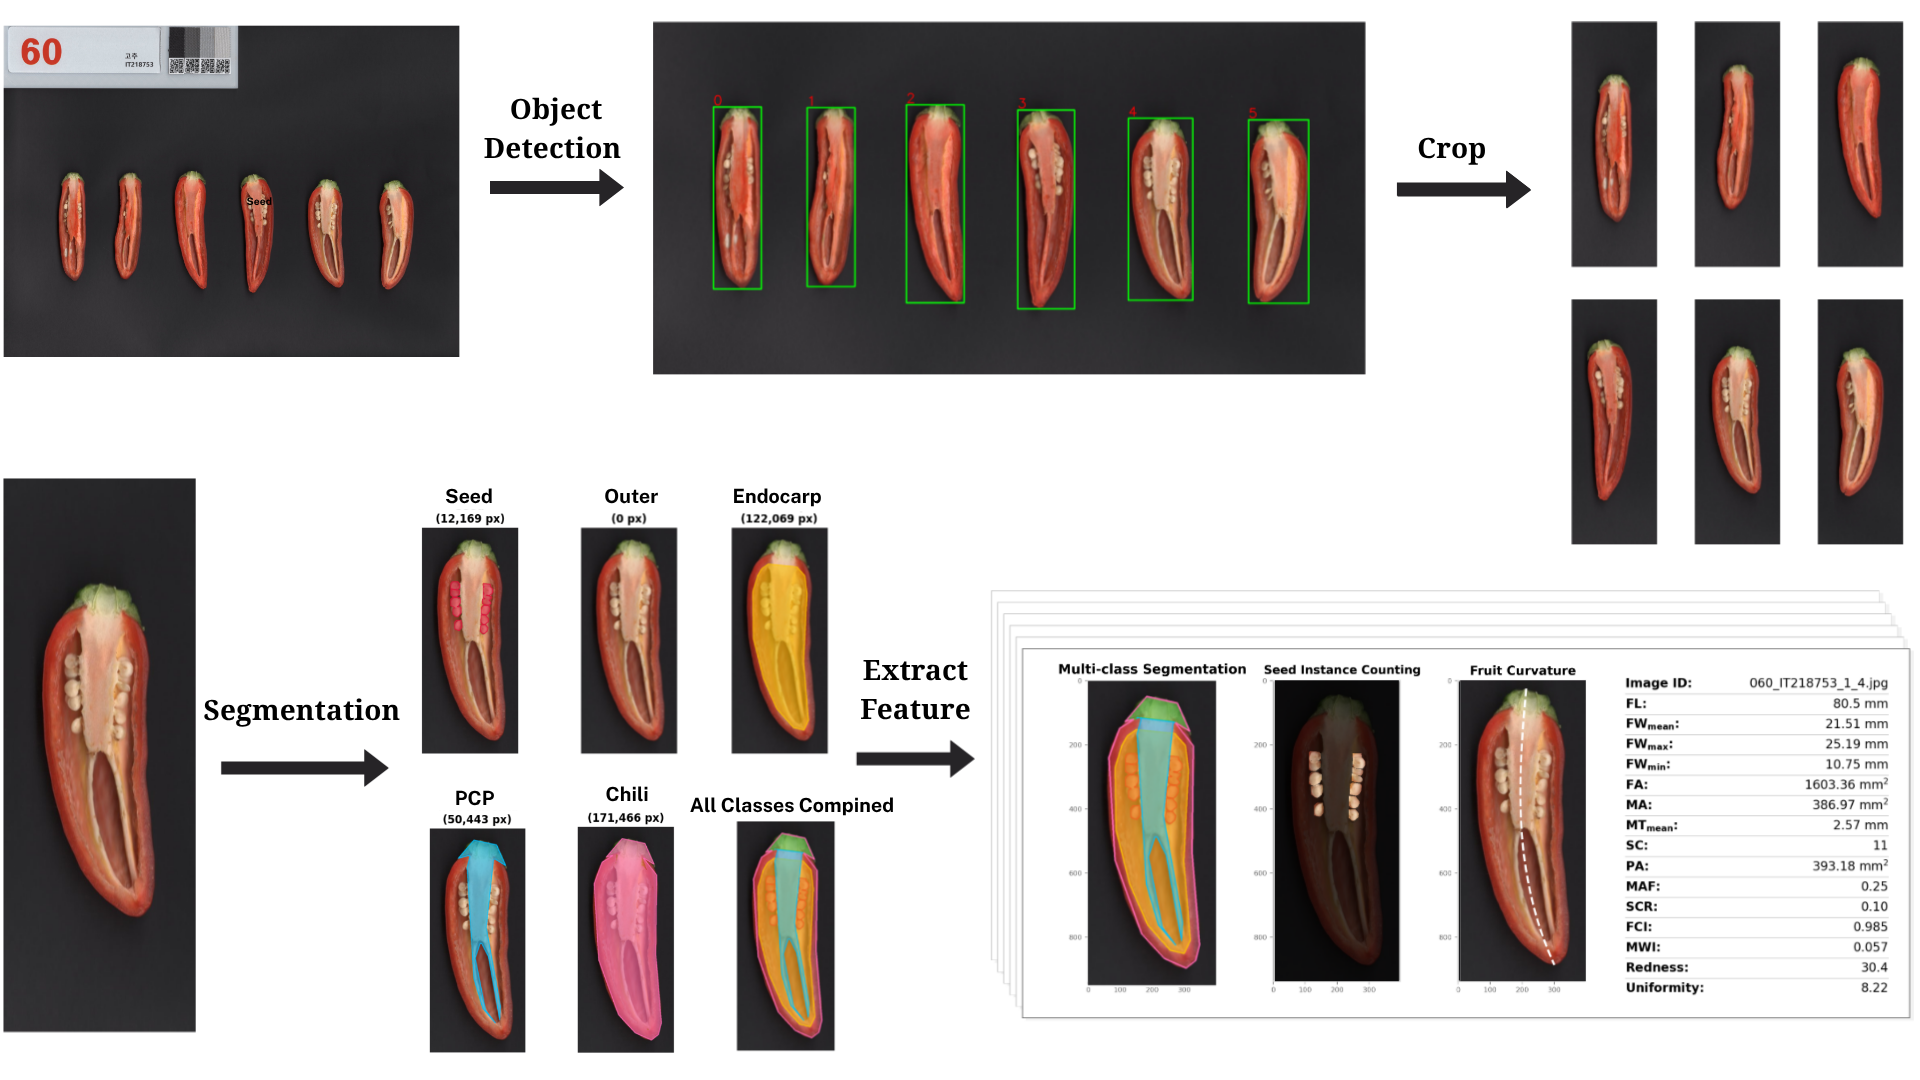
\includegraphics[width=0.9\linewidth,height=0.48\textheight,keepaspectratio]{images/Pipeline_final.png}
\caption[Overall Pipeline]{Overall Pipeline\par\smallskip{\color{viColor}\textbf{VI.} Quy trình tổng thể}}
\label{fig:overall_pipeline}
\end{figure*}



\subsection*{Dataset and plant materials / {\color{viColor} Bộ dữ liệu và vật liệu thực vật}}
The initial plant material comprised 386 chili pepper (\textit{Capsicum annuum}) accessions from the Korean Gene Bank. The accessions were grown under controlled cultivation conditions, with comparable temperature, irrigation, and fertilization regimes maintained to limit environmental influences on phenotypic differences. Within each greenhouse, each accession was assigned to a plot of six plants, with plot positions randomized. The plots were replicated across three separate greenhouses, yielding a total of 18 plants per accession, to limit systematic error and edge effects.

\begin{viet}
Nguồn vật liệu ban đầu của nghiên cứu gồm 386 mẫu nguồn gen ớt (\textit{Capsicum annuum}) từ Ngân hàng Gen Hàn Quốc. Các mẫu được trồng trong điều kiện canh tác được kiểm soát, với nhiệt độ, chế độ tưới và phân bón được duy trì tương đồng nhằm hạn chế ảnh hưởng của môi trường đến sự khác biệt về kiểu hình. Trong mỗi nhà kính, mỗi mẫu nguồn gen được bố trí thành một ô gồm sáu cây, với vị trí các ô được sắp xếp ngẫu nhiên. Các ô được lặp lại tại ba nhà kính khác nhau, tương ứng tổng cộng 18 cây cho mỗi mẫu nguồn gen, nhằm hạn chế sai số hệ thống và hiệu ứng bìa.
\end{viet}




During cultivation and sample collection, some plants died, some accessions on the initial list were not planted, and diseased plants were excluded from sampling. Consequently, usable fruit images were not obtained from all 386 initial accessions. The final dataset comprised 367 original multi-fruit images from 285 accessions. The data were partitioned into training, validation, and test sets at the accession level, ensuring that all images from a given accession belonged to only one set. These sets contained 262, 47, and 58 original images, respectively; after individual-fruit cropping, the corresponding numbers of fruit images were 1237, 264, and 264.

\begin{viet}
Trong quá trình trồng và thu thập mẫu, một số cây bị chết, một số mẫu nguồn gen có trong danh sách ban đầu nhưng không được trồng, và các cây bị bệnh không được lấy mẫu. Vì vậy, không thu được ảnh quả sử dụng được từ toàn bộ 386 mẫu nguồn gen ban đầu. Bộ dữ liệu cuối cùng gồm 367 ảnh gốc chứa nhiều quả, thuộc 285 mẫu nguồn gen. Dữ liệu được chia thành các tập huấn luyện, xác thực và kiểm thử theo mẫu nguồn gen, bảo đảm toàn bộ ảnh của cùng một mẫu nguồn gen chỉ thuộc một tập. Ba tập lần lượt gồm 262, 47 và 58 ảnh gốc; sau khi tách từng quả, số ảnh tương ứng là 1237, 264 và 264.
\end{viet}



\subsection*{Image acquisition and spatial calibration / {\color{viColor} Thu nhận ảnh và hiệu chuẩn không gian}}

Longitudinal fruit sections were photographed under standardized lighting, camera-to-sample distance, and viewing angle to maintain consistency across images. Each image included a white-balance reference patch and a QR code of known dimensions ($10 \times 10$\,mm), used as a calibration reference to convert measurements from pixels to millimetres. When the QR code is detected and decoded, the system determines the conversion factor from its dimensions in the image and its corresponding physical dimensions. If QR decoding fails, the system uses the dataset-level mean scale as a fallback and records the source of the applied scale. The use of a reference object of known dimensions to convert image measurements into physical units is consistent with established methods in plant image analysis \cite{cass}.

\begin{viet}
Các mặt cắt dọc của quả được chụp trong điều kiện chuẩn hóa về ánh sáng, khoảng cách từ camera đến mẫu và góc chụp nhằm duy trì tính nhất quán giữa các ảnh. Mỗi ảnh có kèm một ô tham chiếu cân bằng trắng và mã QR có kích thước đã biết ($10 \times 10$\,mm), được sử dụng làm mốc hiệu chuẩn để quy đổi các phép đo từ pixel sang milimét. Khi phát hiện và giải mã được QR, hệ thống xác định tỷ lệ quy đổi từ kích thước của mốc trên ảnh và kích thước vật lý tương ứng. Nếu không giải mã được QR, hệ thống sử dụng tỷ lệ trung bình của bộ dữ liệu làm phương án dự phòng và ghi nhận nguồn tỷ lệ được áp dụng. Việc sử dụng vật tham chiếu có kích thước đã biết để quy đổi phép đo trên ảnh sang đơn vị vật lý phù hợp với các phương pháp phân tích ảnh thực vật \cite{cass}.
\end{viet}


Letting $(w_{QR}, h_{QR})$ denote the pixel width and height of the decoded QR code's bounding box, the calibration factor $\gamma$ (mm/pixel) is computed as:

\begin{viet}
Gọi $(w_{QR}, h_{QR})$ là chiều rộng và chiều cao tính bằng pixel của hộp giới hạn mã QR đã giải mã; hệ số hiệu chuẩn $\gamma$ (mm/pixel) được tính như sau:
\end{viet}

\begin{equation}
    \gamma = \frac{10}{(w_{QR} + h_{QR})/2} \quad (\text{mm/pixel})
\end{equation}

Using $\gamma$, length and area measurements are converted to their corresponding physical units as follows:

\begin{viet}
Với $\gamma$, các phép đo chiều dài và diện tích được quy đổi sang đơn vị vật lý tương ứng:
\end{viet}

\begin{equation}
 L_{\mathrm{mm}} = L_{\mathrm{px}} \gamma,\qquad
 A_{\mathrm{mm}^2} = A_{\mathrm{px}} \gamma^{2}.
\end{equation}




\noindent Here, $L_{\mathrm{px}}$ is the length in pixels and $A_{\mathrm{px}}$ is the area in pixels$^2$.

\begin{viet}
Trong đó, $L_{\mathrm{px}}$ là chiều dài tính bằng pixel và $A_{\mathrm{px}}$ là diện tích tính bằng pixel$^2$.
\end{viet}



\subsection*{Training Data Preparation and Annotation Protocol / {\color{viColor} Chuẩn bị dữ liệu huấn luyện và quy trình gán nhãn}}
To prepare the segmentation dataset, original images containing multiple fruits were processed to isolate individual longitudinal fruit sections. Fruit localization used a YOLOv7-based object detection model \cite{yolov7}, adopted from a previous study \cite{ver1}. The predicted bounding boxes were expanded with a surrounding margin before cropping to reduce the risk of excluding fruit parts extending beyond the boxes.

\begin{viet}
Để chuẩn bị dữ liệu phân đoạn, các ảnh gốc chứa nhiều quả được xử lý nhằm tách riêng từng mặt cắt quả ớt. Bước định vị sử dụng mô hình phát hiện đối tượng dựa trên YOLOv7 \cite{yolov7}, kế thừa từ nghiên cứu trước \cite{ver1}. Các hộp giới hạn dự đoán được mở rộng thêm một khoảng đệm xung quanh trước khi cắt ảnh nhằm hạn chế việc cắt mất các phần của quả nằm ngoài hộp giới hạn.
\end{viet}


The individual-fruit images were then imported into Label Studio for manual polygon annotation of four target classes:

\begin{viet}
Các ảnh từng quả sau đó được đưa vào Label Studio để gán nhãn thủ công bằng đa giác cho bốn lớp mục tiêu:
\end{viet}

\begin{itemize}
    \item \textbf{Outer}: The part of the fruit outside the cut plane that remains visible in the image due to the three-dimensional structure of the fruit.\par{\color{viColor} \textbf{Outer}: Phần quả nằm ngoài mặt phẳng cắt nhưng vẫn xuất hiện trong ảnh do cấu trúc ba chiều của quả.}
    \item \textbf{Endocarp}: The entire region enclosed by the endocarp boundary in the fruit section, including locations occupied by the placenta and seeds.\par{\color{viColor} \textbf{Endocarp}: Toàn bộ vùng bên trong đường biên nội quả bì trên mặt cắt, bao gồm cả các vị trí có nhau quả và hạt.}
    \item \textbf{PCP (placenta--pedicel composite)}: The composite region comprising the placenta and its attached pedicel.\par{\color{viColor} \textbf{PCP (vùng kết hợp nhau quả--cuống quả)}: Vùng kết hợp nhau quả và phần cuống gắn liền.}
    \item \textbf{Seed}: Seeds were annotated as separate instances according to their visible portions in the image. For overlapping seeds, only the observable portion of each seed was annotated, without inferring occluded regions.\par{\color{viColor} \textbf{Seed}: Các hạt được gán nhãn thành từng thực thể riêng biệt theo phần nhìn thấy trên ảnh. Với các hạt chồng lấp, chỉ phần quan sát được của mỗi hạt được gán nhãn, không suy diễn phần bị che khuất.}
\end{itemize}

For indistinct boundary segments, annotators estimated the boundary position using changes in color, texture, and continuity with neighboring boundary segments. All annotations were reviewed by at least two people to assess consistency and identify annotation errors.

\begin{viet}
Đối với những đoạn đường biên không rõ, người gán nhãn ước lượng vị trí đường biên dựa trên sự thay đổi màu sắc, kết cấu và tính liên tục của các đoạn biên lân cận. Toàn bộ nhãn được ít nhất hai người kiểm tra lại nhằm rà soát tính nhất quán và phát hiện các sai sót trong quá trình gán nhãn.
\end{viet}




\begin{figure}[htbp]
    \centering
    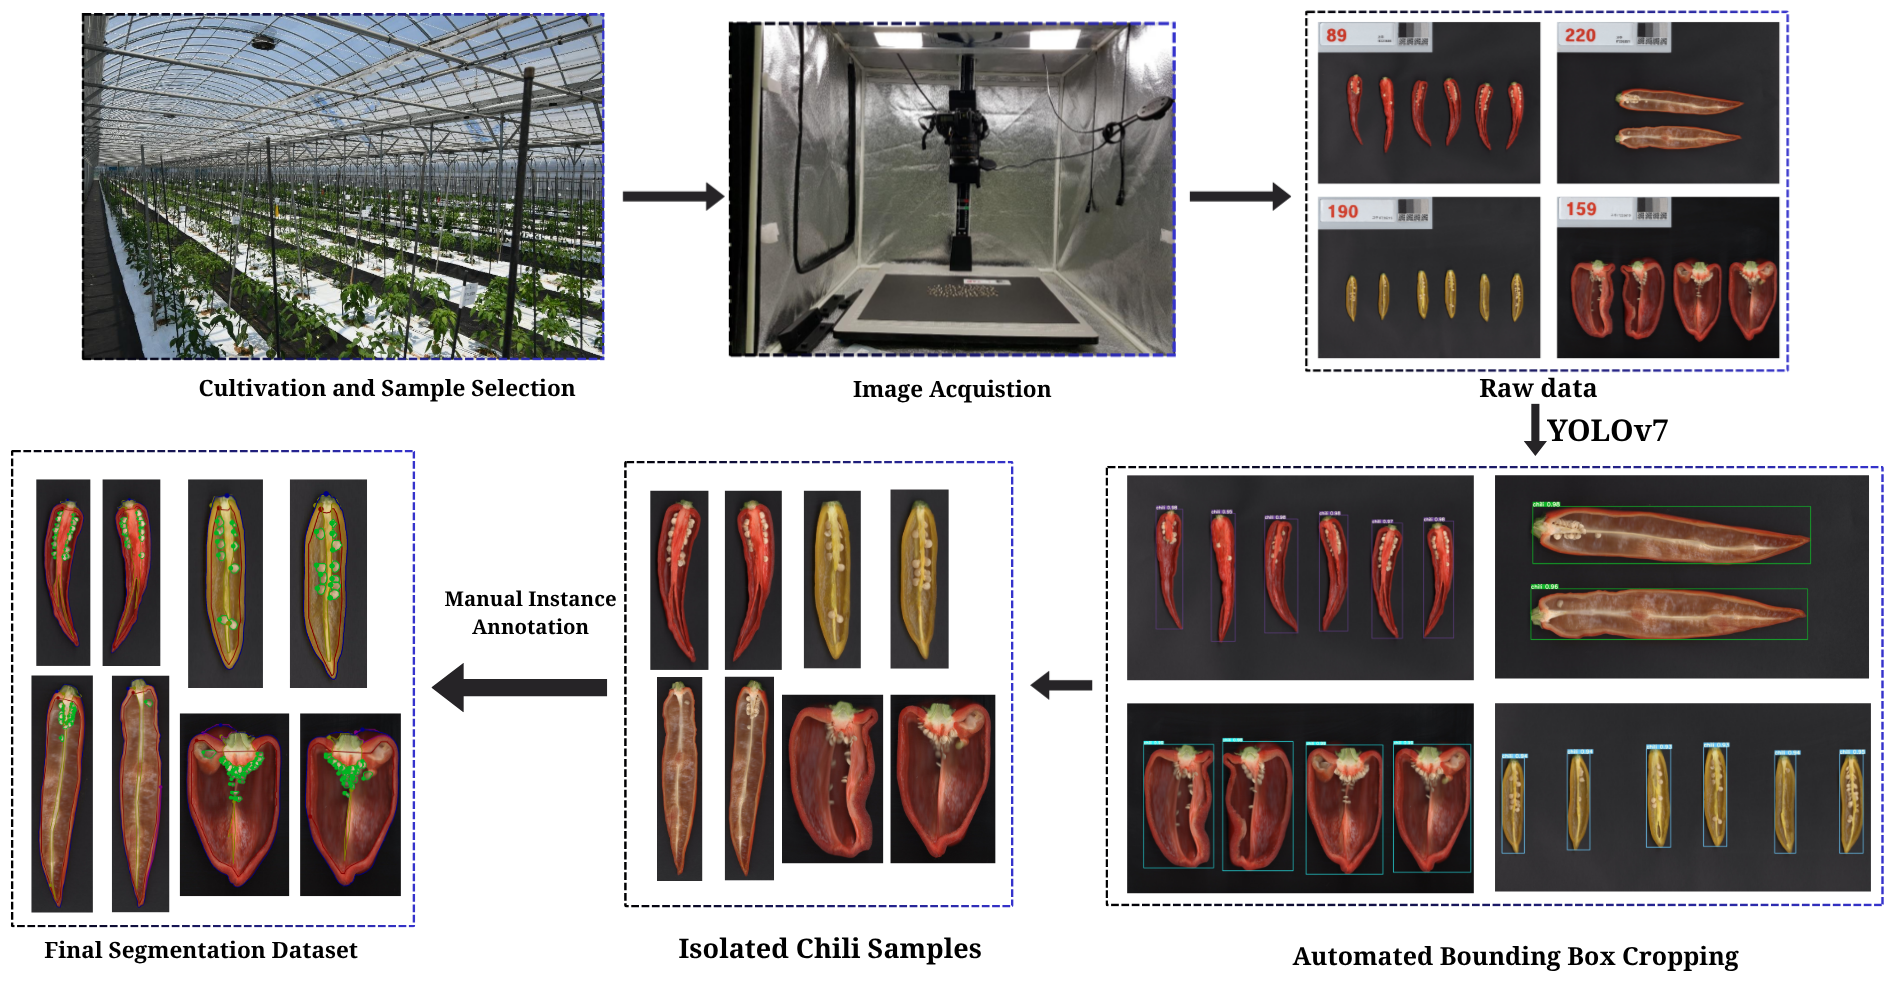
\includegraphics[width=0.9\linewidth,height=0.48\textheight,keepaspectratio]{images/Chili.png}
    \caption[\textbf{Image acquisition and dataset construction workflow for longitudinal chili fruit section segmentation.} The plants were grown in greenhouses, and fruit sections were photographed using a camera system under standardized conditions. From original images containing multiple fruits, YOLOv7 localizes individual fruits with bounding boxes; these boxes are expanded with a surrounding margin before cropping into individual-fruit images. The resulting images are manually annotated using polygons for four classes: outer, endocarp, PCP (placenta--pedicel composite), and seed.]{\textbf{Image acquisition and dataset construction workflow for longitudinal chili fruit section segmentation.} The plants were grown in greenhouses, and fruit sections were photographed using a camera system under standardized conditions. From original images containing multiple fruits, YOLOv7 localizes individual fruits with bounding boxes; these boxes are expanded with a surrounding margin before cropping into individual-fruit images. The resulting images are manually annotated using polygons for four classes: outer, endocarp, PCP (placenta--pedicel composite), and seed.\par\smallskip{\color{viColor}\textbf{VI.} \textbf{Quy trình thu nhận ảnh và xây dựng bộ dữ liệu phân đoạn mặt cắt dọc quả ớt.} Các mẫu được trồng trong nhà kính và chụp bằng hệ thống camera trong điều kiện chuẩn hóa. Từ ảnh gốc chứa nhiều quả, mô hình YOLOv7 định vị từng quả bằng hộp giới hạn; các hộp được mở rộng thêm khoảng đệm trước khi cắt thành ảnh riêng lẻ. Các ảnh sau đó được gán nhãn thủ công bằng đa giác cho bốn lớp: outer, endocarp, PCP (vùng kết hợp nhau quả--cuống quả) và seed.}}
    \label{fig:preprocessing_workflow}
\end{figure}


\subsection*{Instance segmentation model and training configuration / {\color{viColor} Mô hình phân đoạn thực thể và cấu hình huấn luyện}}
This study uses YOLOv8m-seg [REF] to segment four target classes in individual chili fruit images. The model is initialized with weights pretrained on the COCO dataset [REF] and fine-tuned on the annotated dataset of this study. The training, validation, and test sets follow the accession-level partitioning described in the dataset section. During training, data augmentations include horizontal flipping, vertical flipping, rotation within $\pm15^{\circ}$, and Mosaic. All models in the architecture comparison in Section 3.1 are trained and evaluated using the same input size, configured as \texttt{imgsz=960}.

\begin{viet}
Nghiên cứu sử dụng YOLOv8m-seg [REF] để phân đoạn bốn lớp mục tiêu trên ảnh từng quả ớt. Mô hình được khởi tạo từ trọng số huấn luyện trước trên bộ dữ liệu COCO [REF] và tinh chỉnh trên bộ dữ liệu đã gán nhãn của nghiên cứu. Các tập huấn luyện, xác thực và kiểm thử được sử dụng theo cách phân chia theo mẫu nguồn gen đã trình bày ở phần bộ dữ liệu. Trong quá trình huấn luyện, các phép tăng cường dữ liệu gồm lật ngang, lật dọc, xoay trong khoảng $\pm15^{\circ}$ và Mosaic được áp dụng. Tất cả mô hình trong thí nghiệm so sánh kiến trúc tại Mục 3.1 đều được huấn luyện và đánh giá với cùng kích thước đầu vào, được cấu hình ở mức \texttt{imgsz=960}.
\end{viet}


\subsection*{Inference and Mask Generation for Trait Extraction / {\color{viColor} Suy luận và tạo mask phục vụ trích xuất đặc trưng}}

The inference pipeline converts an input image containing multiple fruits into individual-fruit images and their corresponding structural masks, providing the basis for phenotypic trait extraction. The system combines fruit localization using YOLOv7, instance segmentation using YOLOv8m-seg, and a thresholding method adopted from the previous study to generate the whole-fruit mask. Together, these outputs describe the fruit extent and anatomical components, supporting the construction of measurement regions appropriate for each trait.

\begin{viet}
Quy trình suy luận chuyển ảnh đầu vào chứa nhiều quả thành ảnh từng quả cùng các mask cấu trúc tương ứng, làm cơ sở cho việc trích xuất đặc trưng kiểu hình. Hệ thống kết hợp định vị quả bằng YOLOv7, phân đoạn thực thể bằng YOLOv8m-seg và phương pháp phân ngưỡng kế thừa từ nghiên cứu trước để tạo mask toàn quả. Các kết quả này cung cấp thông tin về phạm vi quả và các thành phần giải phẫu, phục vụ xây dựng vùng đo phù hợp cho từng đặc trưng.
\end{viet}

First, YOLOv7 localizes individual fruits in the input image. For the standardized image layout used in this study, the header region containing labels and the calibration marker is excluded from the fruit search region. The remaining image region is resized while preserving its aspect ratio and padded to match the model input. Predicted bounding boxes are filtered by confidence and overlap to remove duplicate detections. The retained boxes are expanded with a surrounding margin before cropping to reduce the risk of excluding fruit parts extending beyond the boxes.

\begin{viet}
Trước tiên, YOLOv7 định vị từng quả trong ảnh đầu vào. Với bố cục ảnh chuẩn hóa của nghiên cứu, vùng đầu ảnh chứa nhãn và mốc hiệu chuẩn được loại khỏi vùng tìm kiếm quả. Vùng ảnh còn lại được thay đổi kích thước theo tỷ lệ và bổ sung phần đệm để phù hợp với đầu vào của mô hình. Các hộp giới hạn dự đoán được lọc theo độ tin cậy và mức độ chồng lấp nhằm loại bỏ phát hiện trùng lặp. Những hộp được giữ lại được mở rộng thêm khoảng đệm trước khi cắt ảnh, nhằm hạn chế việc cắt mất các phần của quả nằm ngoài hộp giới hạn.
\end{viet}

Each individual-fruit image is then processed by YOLOv8m-seg to segment four target classes: outer, endocarp, PCP, and seed. Predictions are filtered by confidence and overlap and then converted into the corresponding binary masks: $M_{\mathrm{outer}}$ represents the fruit region outside the cut plane; $M_{\mathrm{endocarp}}$ represents the region segmented by the model as endocarp; $M_{\mathrm{PCP}}$ represents the composite placenta--pedicel region; and $M_{\mathrm{seed}}$ represents the union of the retained seed regions. Individual seed instance masks are also stored separately for subsequent seed-count estimation.

\begin{viet}
Từng ảnh quả sau đó được xử lý bằng YOLOv8m-seg để phân đoạn bốn lớp mục tiêu: outer, endocarp, PCP và seed. Các dự đoán được lọc theo độ tin cậy và mức độ chồng lấp, sau đó được chuyển thành các mask nhị phân tương ứng: $M_{\mathrm{outer}}$ biểu diễn vùng quả nằm ngoài mặt phẳng cắt; $M_{\mathrm{endocarp}}$ biểu diễn vùng được mô hình phân đoạn thuộc lớp endocarp; $M_{\mathrm{PCP}}$ biểu diễn vùng kết hợp nhau quả--cuống quả; và $M_{\mathrm{seed}}$ biểu diễn hợp các vùng hạt được giữ lại. Các mask của từng thực thể hạt cũng được lưu riêng để phục vụ bước ước lượng số hạt.
\end{viet}

The initial segmentation also supports orientation normalization of elongated, horizontally positioned fruits. For an image whose width exceeds 1.5 times its height and for which a PCP prediction is available, the centroid of the largest PCP instance determines the rotation direction: the image is rotated by $90^{\circ}$ clockwise if the centroid lies in the left half, or counterclockwise if it lies in the right half. Segmentation is repeated on the rotated image to obtain masks corresponding to the new orientation. Images that do not meet these conditions retain their original orientation; the pipeline does not apply a $180^{\circ}$ rotation.

\begin{viet}
Kết quả phân đoạn ban đầu đồng thời được sử dụng để chuẩn hóa hướng của các quả kéo dài nằm ngang. Với ảnh có chiều rộng lớn hơn 1,5 lần chiều cao và có dự đoán PCP, trọng tâm của thực thể PCP lớn nhất được dùng để xác định chiều xoay: ảnh được xoay $90^{\circ}$ theo chiều kim đồng hồ nếu trọng tâm nằm ở nửa trái, hoặc ngược chiều kim đồng hồ nếu nằm ở nửa phải. Mô hình phân đoạn được áp dụng lại trên ảnh đã xoay để thu nhận các mask tương ứng với hướng mới. Những ảnh không đáp ứng điều kiện trên được giữ nguyên hướng; quy trình không thực hiện phép xoay $180^{\circ}$.
\end{viet}

Following orientation normalization, the whole-fruit mask $M_{\mathrm{chili}}$ is generated independently using the red-channel thresholding method adopted from the previous study \cite{ver1}. The thresholded mask undergoes morphological closing, after which the largest external contour is retained and filled to obtain $M_{\mathrm{chili}}$. This mask represents the whole-fruit extent and may include both the outer region and the pedicel.

\begin{viet}
Trên ảnh sau bước chuẩn hóa hướng, mask toàn quả $M_{\mathrm{chili}}$ được tạo độc lập bằng phương pháp phân ngưỡng kênh đỏ kế thừa từ nghiên cứu trước \cite{ver1}. Mask sau phân ngưỡng được xử lý bằng phép đóng hình thái, sau đó giữ và tô kín đường bao ngoài có diện tích lớn nhất để thu được $M_{\mathrm{chili}}$. Mask này biểu diễn phạm vi toàn quả và có thể bao gồm cả vùng outer và cuống.
\end{viet}

The masks $M_{\mathrm{outer}}$, $M_{\mathrm{endocarp}}$, $M_{\mathrm{PCP}}$, and $M_{\mathrm{seed}}$ are clipped to $M_{\mathrm{chili}}$ before subsequent processing. The mask $M_{\mathrm{PCP}}$ is processed to separate the pedicel from the placenta using the method described in the next subsection. The whole-fruit and component masks are then combined according to the requirements of each measurement to construct the mesocarp region, the placenta region, and the fruit-body mask. This combination builds on the thresholding method of the previous study while incorporating anatomical information to expand the trait set and refine existing measurements.

\begin{viet}
Các mask $M_{\mathrm{outer}}$, $M_{\mathrm{endocarp}}$, $M_{\mathrm{PCP}}$ và $M_{\mathrm{seed}}$ được giới hạn trong $M_{\mathrm{chili}}$ trước khi chuyển sang các bước xử lý tiếp theo. Mask $M_{\mathrm{PCP}}$ được xử lý để tách cuống khỏi nhau quả theo phương pháp trình bày ở mục kế tiếp. Mask toàn quả và các mask thành phần sau đó được kết hợp theo yêu cầu của từng phép đo để xây dựng vùng trung quả bì, vùng nhau quả và mask thân quả. Cách kết hợp này tận dụng phương pháp phân ngưỡng của nghiên cứu trước, đồng thời bổ sung thông tin cấu trúc giải phẫu để mở rộng tập đặc trưng và hiệu chỉnh các phép đo đã có.
\end{viet}

\subsection*{Post-segmentation Pedicel Separation / {\color{viColor} Tách cuống quả sau phân đoạn}}
The system separates the pedicel from $M_{\mathrm{PCP}}$ after segmentation to construct the placenta mask and support the definition of the fruit-body cross-sectional region for measurement. The primary separation method uses concave points along the PCP boundary to estimate the junction between the pedicel and placenta, as illustrated in Fig.~\ref{fig:pedicel_separation}A.

\begin{viet}
Hệ thống thực hiện bước tách cuống khỏi $M_{\mathrm{PCP}}$ sau phân đoạn để xây dựng mask nhau quả và hỗ trợ xác định vùng mặt cắt thân quả phục vụ đo lường. Phương pháp tách chính sử dụng các điểm lõm trên đường biên PCP để ước lượng ranh giới giữa cuống và nhau quả, như minh họa ở Hình~\ref{fig:pedicel_separation}A.
\end{viet}


The algorithm extracts the external contour of the PCP mask and divides it into left and right lateral chains. Along each chain, the local turning angle and concavity are evaluated to identify candidate points at the pedicel--placenta junction. A pair of points is selected according to horizontal separation and vertical offset criteria. The contour segments on the pedicel side and the line joining the selected points enclose the estimated pedicel region, which is intersected with the PCP mask to obtain $M_{\mathrm{pedicel}}$.

\begin{viet}
Thuật toán trích xuất contour ngoài của mask PCP và chia đường biên thành hai nhánh bên trái và bên phải. Trên mỗi nhánh, góc đổi hướng và độ lõm cục bộ được đánh giá để xác định các điểm ứng viên tại vùng nối cuống--nhau quả. Một cặp điểm được lựa chọn theo các điều kiện về khoảng cách ngang và độ lệch dọc. Các đoạn đường biên phía cuống cùng đường nối hai điểm được chọn tạo thành vùng cuống ước lượng; vùng này được lấy giao với mask PCP để thu được $M_{\mathrm{pedicel}}$.
\end{viet}




The placenta mask is obtained by subtracting the pedicel region from the PCP mask:

\begin{viet}
Mask nhau quả được xác định bằng cách loại vùng cuống khỏi mask PCP:
\end{viet}

\begin{equation}
    M_{\mathrm{placenta}} = M_{\mathrm{PCP}} \setminus M_{\mathrm{pedicel}}.
\end{equation}
Here, $M_{\mathrm{pedicel}}$ is the pedicel mask and $M_{\mathrm{placenta}}$ is the estimated placenta mask. These masks are used in measurements involving placenta area and the fruit-body cross-sectional region.

\begin{viet}
Trong đó, $M_{\mathrm{pedicel}}$ là mask cuống và $M_{\mathrm{placenta}}$ là mask nhau quả ước lượng. Các mask này được sử dụng trong những phép đo liên quan đến diện tích nhau quả và vùng mặt cắt thân quả.
\end{viet}



\begin{figure}[htbp]
\centering
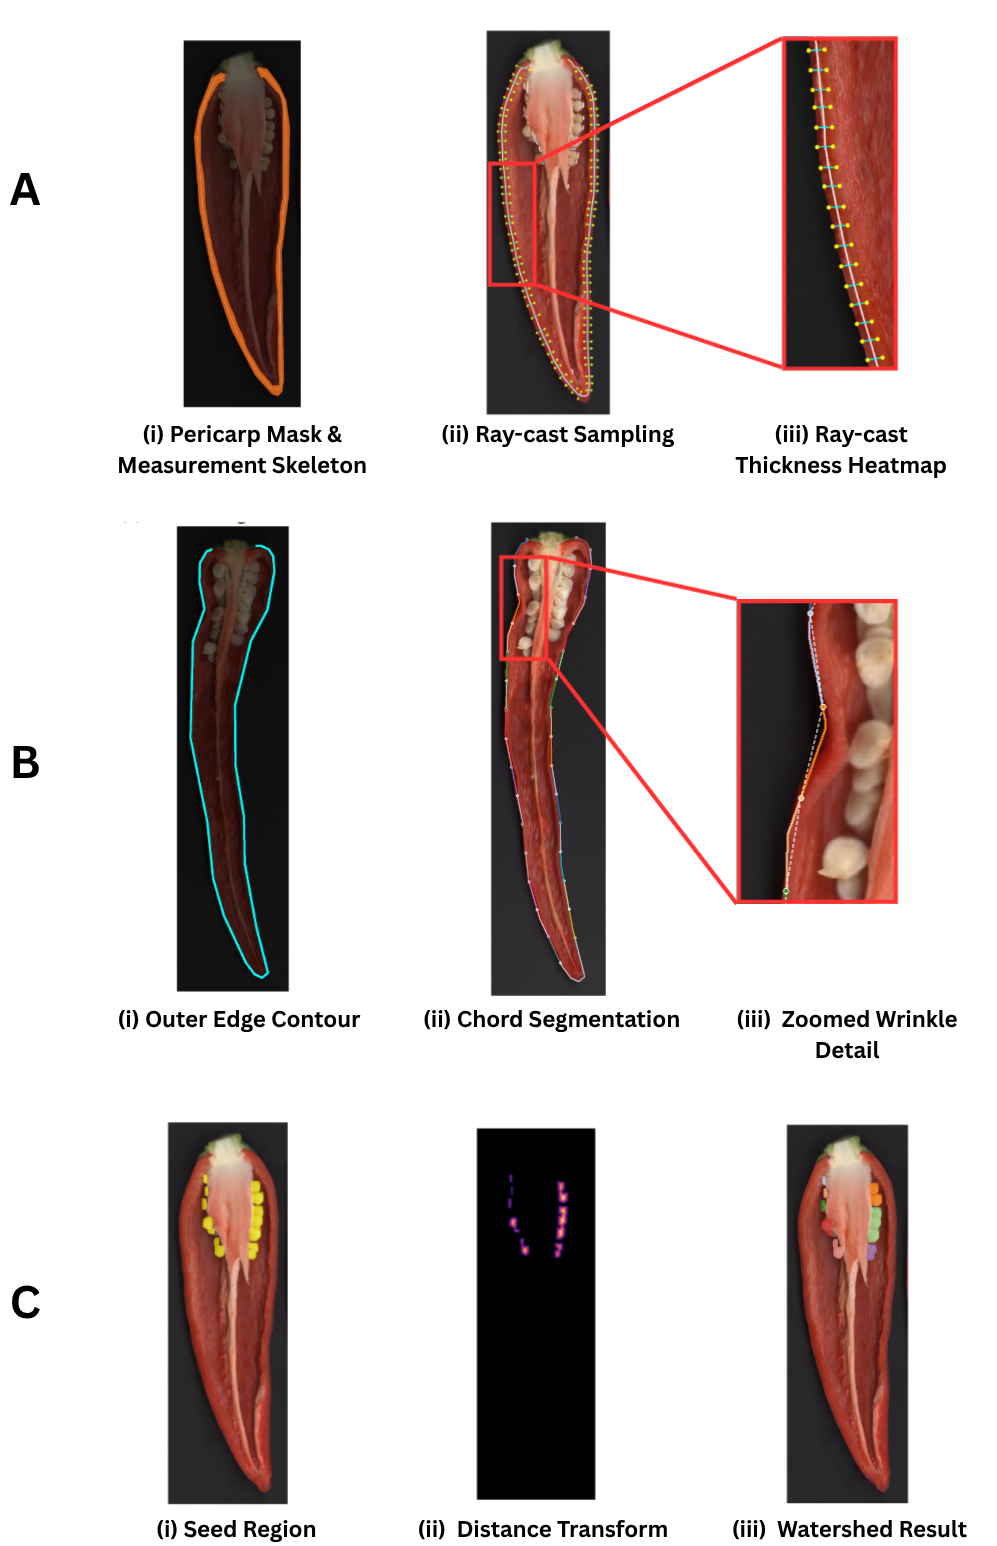
\includegraphics[width=0.9\linewidth,height=0.48\textheight,keepaspectratio]{images/pedicel_placeholder.png}
\caption[Pedicel separation illustration (draft)]{\textbf{Draft placeholder for the mask-processing illustration.} Planned panel (A): pedicel separation from the PCP mask. Panels (B) and (C): to be determined. The image is temporarily copied from Fig.~\ref{fig:method_thickness_wrinkle_seed} and does not yet illustrate the planned panels.\par\smallskip{\color{viColor}\textbf{VI.} \textbf{Hình tạm cho minh họa xử lý mask.} Nội dung dự kiến của (A): tách cuống khỏi mask PCP. (B) và (C): chưa xác định. Ảnh hiện được sao chép tạm từ Hình~\ref{fig:method_thickness_wrinkle_seed}, chưa minh họa nội dung dự kiến.}}
\label{fig:pedicel_separation}
\end{figure}

\begin{figure}[htbp]
\centering
% Replace with your actual image path
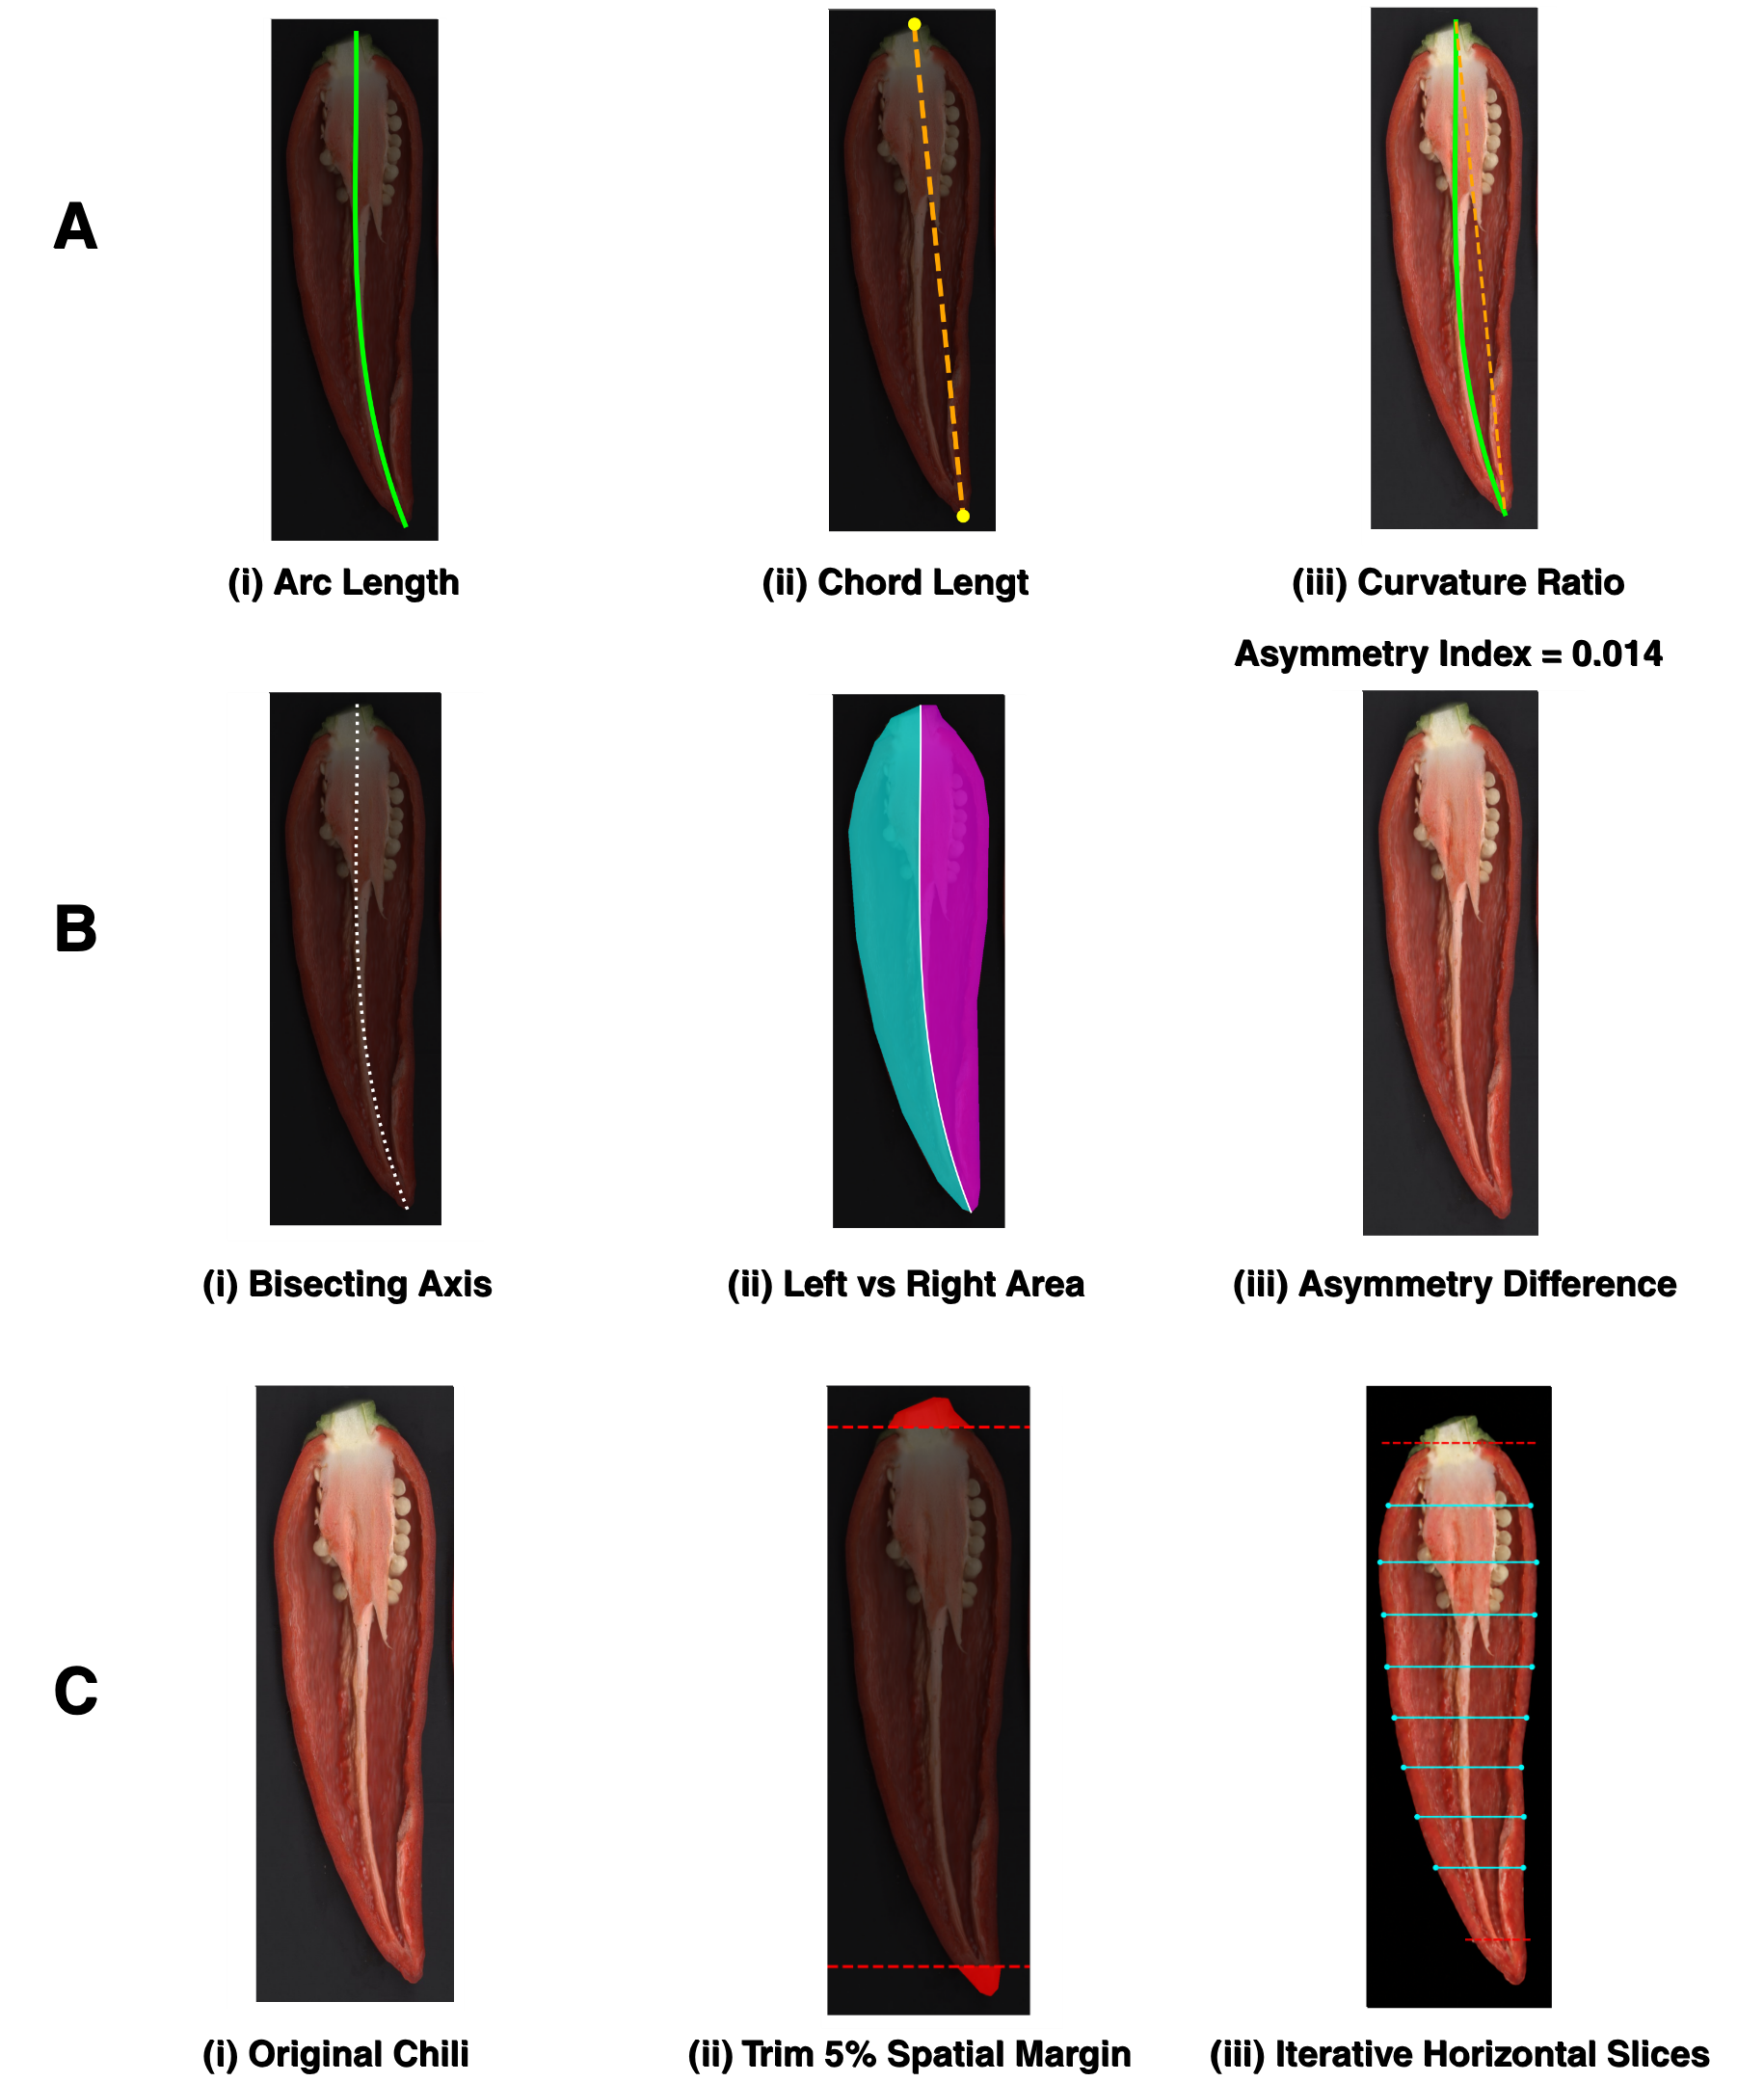
\includegraphics[width=0.9\linewidth,height=0.48\textheight,keepaspectratio]{images/fig_1.png}
\caption[\textbf{Geometric feature extraction for fruit curvature, fruit asymmetry, and mean fruit width.} (A) The Fruit Curvature Index ($FCI$) captures global bending as one minus the regularized ratio of the endpoint chord length to the fitted fruit-body spine length; values near zero indicate a nearly straight axis, and larger values indicate greater bending. (B) Left and right widths are compared relative to the straight line joining the endpoints of the fitted fruit-body spine to derive maximum leftward, maximum rightward, and mean signed deviation. (C) Mean Fruit Width ($FW_{\mathrm{mean}}$) is calculated as the average of eight horizontal chords measured at the interior scanlines among ten equally spaced scanlines spanning the fruit-mask extent.]{\textbf{Geometric feature extraction for fruit curvature, fruit asymmetry, and mean fruit width.} (A) The Fruit Curvature Index ($FCI$) captures global bending as one minus the regularized ratio of the endpoint chord length to the fitted fruit-body spine length; values near zero indicate a nearly straight axis, and larger values indicate greater bending. (B) Left and right widths are compared relative to the straight line joining the endpoints of the fitted fruit-body spine to derive maximum leftward, maximum rightward, and mean signed deviation. (C) Mean Fruit Width ($FW_{\mathrm{mean}}$) is calculated as the average of eight horizontal chords measured at the interior scanlines among ten equally spaced scanlines spanning the fruit-mask extent.\par\smallskip{\color{viColor}\textbf{VI.} \textbf{Trích xuất đặc trưng hình học cho độ cong, tính bất đối xứng và chiều rộng trung bình của quả.} (A) Chỉ số độ cong quả ($FCI$) mô tả độ uốn tổng thể bằng một trừ tỷ số giữa chiều dài dây cung nối hai đầu đường trục thân quả và chiều dài đường trục, với hằng số nhỏ được thêm vào cả tử và mẫu; giá trị gần 0 biểu thị trục gần thẳng, còn giá trị lớn hơn biểu thị độ uốn lớn hơn. (B) Chiều rộng trái và phải được so sánh quanh đường thẳng nối hai đầu đường trục thân quả đã khớp để xác định độ lệch trái lớn nhất, độ lệch phải lớn nhất và độ lệch trung bình có dấu. (C) Chiều rộng quả trung bình ($FW_{\mathrm{mean}}$) được tính bằng trung bình tám dây cung ngang đo tại các đường quét bên trong của mười đường quét cách đều nhau trải trên phạm vi mask quả.}}
\label{fig:method_curvature_asym_width}
\end{figure}

\subsection*{Extract Fruit Area ($FA$) / {\color{viColor} Trích xuất diện tích quả ($FA$)}}

Fruit area ($FA$) is measured on the fruit-body mask, obtained by removing the outer region and the separated pedicel from the whole-fruit mask:

\begin{viet}
Diện tích quả ($FA$) được đo trên mask thân quả, được tạo bằng cách loại vùng outer và phần cuống đã tách khỏi mask toàn quả:
\end{viet}

\begin{equation}
M_{\mathrm{body}}=M_{\mathrm{chili}}\setminus\left(M_{\mathrm{pedicel}}\cup M_{\mathrm{outer}}\right).
\end{equation}

Here, $M_{\mathrm{body}}$ is the binary fruit-body mask. Fruit area is calculated as:

\begin{viet}
Trong đó, $M_{\mathrm{body}}$ là mask nhị phân của thân quả. Diện tích quả được tính như sau:
\end{viet}

\begin{equation}
FA=\gamma^2|M_{\mathrm{body}}|.
\end{equation}

Here, $FA$ is Fruit Area in mm$^2$. Throughout the mask-area formulas, $|M|$ denotes the number of foreground pixels belonging to the binary mask $M$ (pixels with nonzero mask values). Thus, $|M_{\mathrm{body}}|$ counts the pixels in the fruit-body mask. Multiplication by $\gamma^2$ converts this pixel count to area in mm$^2$.

\begin{viet}
Trong đó, $FA$ là diện tích quả tính bằng mm$^2$. Trong các công thức diện tích mask, $|M|$ biểu diễn số pixel tiền cảnh thuộc mask nhị phân $M$ (các pixel có giá trị mask khác 0). Do đó, $|M_{\mathrm{body}}|$ là số pixel thuộc mask thân quả. Nhân số pixel này với $\gamma^2$ sẽ thu được diện tích theo mm$^2$.
\end{viet}

\subsection*{Extraction of Fruit Length ($FL$) and Fruit Width ($FW$) / {\color{viColor} Trích xuất chiều dài quả ($FL$) và chiều rộng quả ($FW$)}}

The fitted central spine used for fruit-length estimation is illustrated in Fig.~\ref{fig:method_curvature_asym_width}A. Fruit length is estimated from a central spine fitted to the previously defined fruit-body mask $M_{\mathrm{body}}$.

\begin{viet}
Đường trục trung tâm đã khớp dùng để ước lượng chiều dài quả được minh họa ở Hình~\ref{fig:method_curvature_asym_width}A. Chiều dài quả được ước lượng từ đường trục trung tâm khớp với mask thân quả $M_{\mathrm{body}}$ đã định nghĩa ở trên.
\end{viet}

For each nonempty image row of $M_{\mathrm{body}}$, the midpoint between the leftmost and rightmost foreground pixels is calculated. A third-degree polynomial, $x=f_3(y)$, is fitted to these midpoints, where $y$ is the image-row coordinate and $f_3(y)$ gives the horizontal coordinate of the fitted central spine at that row. The spine arc length is approximated by a discrete sum over the valid pixel rows:

\begin{viet}
Với mỗi hàng ảnh không rỗng của $M_{\mathrm{body}}$, trung điểm giữa pixel tiền cảnh ngoài cùng bên trái và bên phải được tính toán. Một đa thức bậc ba, $x=f_3(y)$, được khớp với các trung điểm này, trong đó $y$ là tọa độ hàng ảnh và $f_3(y)$ biểu diễn tọa độ ngang của đường trục trung tâm đã khớp tại hàng đó. Độ dài cung của đường trục được xấp xỉ bằng tổng rời rạc trên các hàng pixel hợp lệ:
\end{viet}


\begin{equation}
 FL\approx\gamma\sum_{y\in\mathcal{Y}_{\mathrm{spine}}}\sqrt{1+\left[f'_3(y)\right]^2}\,\Delta y,\qquad\Delta y=1\text{ pixel}.
\end{equation}
Here, $\mathcal{Y}_{\mathrm{spine}}$ is the set of nonempty rows of $M_{\mathrm{body}}$ and $f'_3(y)$ is the first derivative of the fitted polynomial. Fruit length is rounded to two decimal places.

\begin{viet}
Trong đó, $\mathcal{Y}_{\mathrm{spine}}$ là tập các hàng không rỗng của $M_{\mathrm{body}}$, $f'_3(y)$ là đạo hàm bậc nhất của đa thức đã khớp. Chiều dài quả được làm tròn đến hai chữ số thập phân.
\end{viet}


The horizontal scanlines used for fruit-width measurement are illustrated in Fig.~\ref{fig:method_curvature_asym_width}C. Fruit width is measured directly from the fruit mask using horizontal
scanlines. Ten equally spaced scanlines span the mask's occupied vertical
extent, dividing it into nine equal intervals:

\begin{viet}
Các đường quét ngang dùng để đo chiều rộng quả được minh họa ở Hình~\ref{fig:method_curvature_asym_width}C. Chiều rộng quả được đo trực tiếp từ mask quả bằng các đường quét ngang. Mười đường quét cách đều nhau trải trên toàn bộ phạm vi theo phương dọc mà mask chiếm giữ, chia phạm vi này thành chín khoảng bằng nhau:
\end{viet}

\begin{equation}
    y_k = \operatorname{round}\left(
    y_{\min}^{\mathrm{mask}} +
    \frac{k}{9}\left(y_{\max}^{\mathrm{mask}}-y_{\min}^{\mathrm{mask}}\right)
    \right), \qquad k=0,\ldots,9.
\end{equation}
Here, $y_{\min}^{\mathrm{mask}}$ and $y_{\max}^{\mathrm{mask}}$ are the topmost and bottommost image-row coordinates occupied by the fruit mask, respectively; $y_k$ is the row coordinate of scanline $k$, and $\operatorname{round}$ rounds to the nearest integer pixel row.

\begin{viet}
Trong đó, $y_{\min}^{\mathrm{mask}}$ và $y_{\max}^{\mathrm{mask}}$ lần lượt là tọa độ hàng trên cùng và dưới cùng có pixel thuộc mask quả; $y_k$ là tọa độ hàng của đường quét thứ $k$, còn $\operatorname{round}$ làm tròn về hàng pixel nguyên gần nhất.
\end{viet}

The two endpoint scanlines are excluded. At each of the eight interior
scanlines, $k=1,\ldots,8$, the horizontal chord extends from the leftmost
to the rightmost foreground pixel of the fruit mask. Its physical width is

\begin{viet}
Hai đường quét ở hai đầu được loại bỏ. Tại mỗi đường trong số tám đường quét bên trong, $k=1,\ldots,8$, dây cung ngang kéo dài từ pixel tiền cảnh ngoài cùng bên trái đến pixel tiền cảnh ngoài cùng bên phải của mask quả. Chiều rộng vật lý tương ứng là:
\end{viet}

\begin{equation}
    FW_k = \gamma\left(x_{\mathrm{right}}(y_k)
    - x_{\mathrm{left}}(y_k)\right).
\end{equation}
Here, $x_{\mathrm{left}}(y_k)$ and $x_{\mathrm{right}}(y_k)$ are the horizontal pixel coordinates of the leftmost and rightmost foreground pixels at row $y_k$, respectively, and $FW_k$ is the corresponding fruit width in mm.

\begin{viet}
Trong đó, $x_{\mathrm{left}}(y_k)$ và $x_{\mathrm{right}}(y_k)$ lần lượt là tọa độ ngang tính bằng pixel của pixel tiền cảnh ngoài cùng bên trái và bên phải tại hàng $y_k$; $FW_k$ là chiều rộng quả tương ứng tính bằng mm.
\end{viet}

The minimum, mean, and maximum fruit widths are calculated from these eight
measurements:

\begin{viet}
Chiều rộng quả nhỏ nhất, trung bình và lớn nhất được tính từ tám phép đo này:
\end{viet}

\begin{align}
    FW_{\min} &= \min_{k=1,\ldots,8} FW_k, \\
    FW_{\mathrm{mean}} &= \frac{1}{8}\sum_{k=1}^{8} FW_k, \\
    FW_{\max} &= \max_{k=1,\ldots,8} FW_k.
\end{align}
Here, $FW_{\min}$, $FW_{\mathrm{mean}}$, and $FW_{\max}$ are the minimum, mean, and maximum fruit widths measured at the eight interior scanlines, respectively, all in mm.

\begin{viet}
Trong đó, $FW_{\min}$, $FW_{\mathrm{mean}}$ và $FW_{\max}$ lần lượt là chiều rộng quả nhỏ nhất, trung bình và lớn nhất tại tám đường quét bên trong, đều tính bằng mm.
\end{viet}


\subsection*{Extract Fruit Curvature Index ($FCI$) / {\color{viColor} Trích xuất chỉ số độ cong quả ($FCI$)}}
The Fruit Curvature Index ($FCI$) describes the overall bending of the fruit body through the relationship between the straight-line distance connecting the spine endpoints and the spine length. It uses the spine $x=f_3(y)$ fitted to $M_{\mathrm{body}}$ during fruit-length estimation, as illustrated in Fig.~\ref{fig:method_curvature_asym_width}A:

\begin{viet}
Chỉ số độ cong quả ($FCI$) mô tả mức độ uốn cong tổng thể của thân quả thông qua quan hệ giữa khoảng cách thẳng nối hai đầu đường trục và chiều dài đường trục. Phép đo sử dụng đường trục $x=f_3(y)$ đã khớp trên $M_{\mathrm{body}}$ trong bước tính chiều dài quả, như minh họa ở Hình~\ref{fig:method_curvature_asym_width}A:
\end{viet}

\begin{equation}
 FCI=1-\frac{\varepsilon_{\mathrm{C}}+\gamma\sqrt{[f_3(y_{\max})-f_3(y_{\min})]^2+(y_{\max}-y_{\min})^2}}{\varepsilon_{\mathrm{C}}+FL}.
\end{equation}
Here, $y_{\min}$ and $y_{\max}$ are the first and last row coordinates of the fruit-body spine, respectively; $\varepsilon_{\mathrm{C}}=10^{-6}\,\mathrm{mm}$ is a small positive constant that prevents a zero denominator. The square-root expression multiplied by $\gamma$ gives the straight-line distance between the spine endpoints. FCI values near zero indicate a nearly straight spine, whereas values closer to one indicate greater overall bending.

\begin{viet}
Trong đó, $y_{\min}$ và $y_{\max}$ là tọa độ hàng đầu và cuối của đường trục thân quả; $\varepsilon_{\mathrm{C}}=10^{-6}\,\mathrm{mm}$ là hằng số dương nhỏ giúp tránh mẫu số bằng 0. Biểu thức chứa căn bậc hai sau khi nhân với $\gamma$ là chiều dài đoạn thẳng nối hai đầu đường trục. Giá trị FCI gần 0 biểu thị đường trục gần thẳng, trong khi giá trị càng gần 1 biểu thị mức độ uốn cong tổng thể càng lớn.
\end{viet}

\subsection*{Extraction of Deviation / {\color{viColor} Trích xuất độ lệch}}

Left--right deviation of the fruit body is determined by comparing the widths on either side of a common reference line, as illustrated in Fig.~\ref{fig:method_curvature_asym_width}B. Let $x=f_{\mathrm{axis}}(y)$ denote the straight line joining the endpoints of the spine $x=f_3(y)$ fitted to $M_{\mathrm{body}}$ during fruit-length and curvature estimation. At each row $y\in\mathcal{Y}_{\mathrm{spine}}$, the dividing position is constrained to lie between the two boundaries:

\begin{viet}
Độ lệch trái--phải của thân quả được xác định bằng cách so sánh chiều rộng hai phía quanh một đường tham chiếu chung, như minh họa ở Hình~\ref{fig:method_curvature_asym_width}B. Gọi $x=f_{\mathrm{axis}}(y)$ là đường thẳng nối hai đầu đường trục $x=f_3(y)$ đã khớp trên $M_{\mathrm{body}}$ trong bước tính chiều dài và độ cong quả. Tại mỗi hàng $y\in\mathcal{Y}_{\mathrm{spine}}$, vị trí chia hai phía được giới hạn trong khoảng giữa hai biên:
\end{viet}

\begin{equation}
\tilde{x}(y)=\min\!\left[x_{\mathrm{right}}(y),\,\max\!\left(x_{\mathrm{left}}(y),f_{\mathrm{axis}}(y)\right)\right].
\end{equation}

Here, $\tilde{x}(y)$ is the constrained horizontal dividing coordinate; the boundary coordinates in this step are taken from $M_{\mathrm{body}}$. The left and right widths are calculated as:

\begin{viet}
Trong đó, $\tilde{x}(y)$ là tọa độ ngang của vị trí chia sau khi giới hạn; các tọa độ biên tại bước này được lấy trên $M_{\mathrm{body}}$. Chiều rộng bên trái và bên phải được tính như sau:
\end{viet}

\begin{equation}
W_L(y)=\tilde{x}(y)-x_{\mathrm{left}}(y),\qquad W_R(y)=x_{\mathrm{right}}(y)-\tilde{x}(y).
\end{equation}

Here, $W_L(y)$ and $W_R(y)$ are the widths of the fruit body to the left and right of the reference line at row $y$, respectively, in pixels. When the reference line lies outside the boundary span, the full row width is assigned to the side containing the fruit, while the opposite side has zero width. Signed row-wise deviation is normalized by the total width:

\begin{viet}
Trong đó, $W_L(y)$ và $W_R(y)$ lần lượt là chiều rộng phần thân quả nằm bên trái và bên phải đường tham chiếu tại hàng $y$, tính bằng pixel. Khi đường tham chiếu nằm ngoài khoảng giữa hai biên, toàn bộ chiều rộng hàng được gán cho phía chứa quả, còn phía kia có chiều rộng bằng 0. Độ lệch có dấu tại mỗi hàng được chuẩn hóa theo tổng chiều rộng:
\end{viet}

\begin{equation}
d(y)=\frac{W_R(y)-W_L(y)}{W_R(y)+W_L(y)+\varepsilon_{\mathrm{A}}},\qquad y\in\mathcal{Y}_{\mathrm{spine}}.
\end{equation}

Here, $\varepsilon_{\mathrm{A}}=10^{-6}\,\mathrm{pixel}$ is a small positive constant that prevents a zero denominator; a zero-width row therefore has $d(y)=0$. Negative values indicate leftward deviation, positive values indicate rightward deviation, and zero indicates equal widths on both sides. Since $\varepsilon_{\mathrm{A}}>0$, $d(y)\in(-1,1)$; values approach $-1$ or $1$ when the entire row width lies to the left or right of the reference line, respectively. The maximum leftward deviation ($D_L$), maximum rightward deviation ($D_R$), and mean signed deviation ($D_{\mathrm{mean}}$) are calculated as:

\begin{viet}
Trong đó, $\varepsilon_{\mathrm{A}}=10^{-6}\,\mathrm{pixel}$ là hằng số dương nhỏ giúp tránh mẫu số bằng 0; khi chiều rộng hàng bằng 0, $d(y)=0$. Giá trị âm biểu thị lệch trái, giá trị dương biểu thị lệch phải và giá trị bằng 0 biểu thị hai phía cân bằng. Do $\varepsilon_{\mathrm{A}}>0$, $d(y)\in(-1,1)$; giá trị gần $-1$ hoặc $1$ tương ứng với toàn bộ chiều rộng hàng nằm bên trái hoặc bên phải đường tham chiếu. Độ lệch trái lớn nhất ($D_L$), độ lệch phải lớn nhất ($D_R$) và độ lệch trung bình có dấu ($D_{\mathrm{mean}}$) được xác định:
\end{viet}

\begin{equation}
D_L=\min\!\left(0,\min_{y\in\mathcal{Y}_{\mathrm{spine}}}d(y)\right).
\end{equation}

\begin{equation}
D_R=\max\!\left(0,\max_{y\in\mathcal{Y}_{\mathrm{spine}}}d(y)\right).
\end{equation}

\begin{equation}
D_{\mathrm{mean}}=\frac{1}{|\mathcal{Y}_{\mathrm{spine}}|}\sum_{y\in\mathcal{Y}_{\mathrm{spine}}}d(y).
\end{equation}

Here, $|\mathcal{Y}_{\mathrm{spine}}|$ denotes the number of valid image rows. $D_{\mathrm{mean}}$ is calculated by summing the signed deviations $d(y)$ over these rows and dividing by their number. All three indices are dimensionless. $D_L\in(-1,0]$ and $D_R\in[0,1)$ describe the strongest deviation toward each side; zero indicates that no row deviates toward that side. $D_{\mathrm{mean}}\in(-1,1)$ describes the overall directional tendency, with equal weight assigned to each row. A mean near zero does not necessarily imply a symmetric fruit body, because leftward and rightward deviations can cancel.

\begin{viet}
Trong đó, $|\mathcal{Y}_{\mathrm{spine}}|$ là số hàng ảnh hợp lệ. $D_{\mathrm{mean}}$ được tính bằng cách cộng các độ lệch có dấu $d(y)$ trên các hàng này rồi chia cho số hàng tương ứng. Cả ba chỉ số đều không có đơn vị. $D_L\in(-1,0]$ và $D_R\in[0,1)$ biểu diễn mức lệch mạnh nhất về từng phía; giá trị bằng 0 cho biết không có hàng lệch về phía tương ứng. $D_{\mathrm{mean}}\in(-1,1)$ mô tả xu hướng lệch chung, với trọng số bằng nhau cho mỗi hàng. Giá trị trung bình gần 0 không nhất thiết biểu thị thân quả đối xứng, vì các độ lệch trái và phải có thể triệt tiêu nhau.
\end{viet}

\subsection*{Extract Mesocarp Area ($MA$) / {\color{viColor} Trích xuất diện tích trung quả bì ($MA$)}}

To construct the mesocarp mask, the outer mask is first subtracted from the whole-fruit mask. The resulting mask is cleaned by morphological opening and connected-component filtering before the internal anatomical masks are removed. A final component filter suppresses small isolated remnants. Denoting these two cleaning operations by $\mathcal{C}$ and $\mathcal{F}$, respectively, the runtime mask can be written as

\begin{viet}
Để tạo mask trung quả bì, trước tiên mask outer được trừ khỏi mask toàn quả. Mask thu được được làm sạch bằng phép mở hình thái và lọc thành phần liên thông trước khi loại các mask giải phẫu bên trong. Một bước lọc thành phần cuối cùng loại các phần dư nhỏ, tách biệt. Ký hiệu hai thao tác làm sạch này lần lượt là $\mathcal{C}$ và $\mathcal{F}$, mask khi chạy có thể được viết như sau:
\end{viet}

\begin{equation}
 M_{\mathrm{mesocarp}}=\mathcal{F}\!\left[\mathcal{C}(M_{\mathrm{chili}}\setminus M_{\mathrm{outer}})\setminus\left(M_{\mathrm{endocarp}}\cup M_{\mathrm{PCP}}\cup M_{\mathrm{seed}}\right)\right].
\end{equation}
The mesocarp area ($MA$) is therefore:

\begin{viet}
Do đó, diện tích trung quả bì ($MA$) là:
\end{viet}

\begin{equation}
    MA=\gamma^2|M_{\mathrm{mesocarp}}|.
\end{equation}
Here, $MA$ is Mesocarp Area in mm$^2$, and $|M_{\mathrm{mesocarp}}|$ is the number of foreground pixels belonging to the retained mesocarp mask.

\begin{viet}
Trong đó, $MA$ là diện tích trung quả bì tính bằng mm$^2$ và $|M_{\mathrm{mesocarp}}|$ là số pixel tiền cảnh thuộc mask mô trung quả bì được giữ lại.
\end{viet}

\subsection*{Extract Mesocarp Thickness / {\color{viColor} Trích xuất độ dày trung quả bì}}

The mesocarp mask $M_{\mathrm{mesocarp}}$ is additionally smoothed using morphological operations to reduce small boundary irregularities and skeleton branches caused by segmentation noise. The smoothed mask is used consistently to determine the inner and outer boundaries and construct the skeleton for thickness measurement.

\begin{viet}
Mask trung quả bì $M_{\mathrm{mesocarp}}$ được làm trơn bổ sung bằng các phép toán hình thái nhằm giảm những bất thường nhỏ trên biên và hạn chế các nhánh khung xương phát sinh do nhiễu phân đoạn. Mask sau làm trơn được sử dụng thống nhất để xác định đường biên trong, đường biên ngoài và dựng khung xương phục vụ đo độ dày.
\end{viet}

The skeleton represents the medial axis of the mesocarp region. Side branches are removed by retaining the longest geodesic backbone in each skeleton component. Measurement locations $\mathbf{s}_i$ are sampled along the skeleton at an arc-length interval of $1\,\mathrm{mm}$ to distribute measurements along the tissue.

\begin{viet}
Khung xương biểu diễn đường giữa của vùng trung quả bì. Các nhánh phụ được loại bỏ bằng cách giữ lại đường chính có độ dài trắc địa lớn nhất trong mỗi thành phần khung xương. Các vị trí đo $\mathbf{s}_i$ được lấy mẫu dọc theo khung xương với bước độ dài cung $1\,\mathrm{mm}$, giúp phân bố phép đo theo chiều dài vùng mô.
\end{viet}

At each location $\mathbf{s}_i$, straight lines passing through the point are examined in multiple directions. A measurement line is valid when it intersects the inner and outer boundaries on opposite sides of $\mathbf{s}_i$. Among the valid measurement segments, the shortest segment connecting the two intersections is selected as the local mesocarp thickness, as illustrated in Fig.~\ref{fig:method_thickness_wrinkle_seed}A:

\begin{viet}
Tại mỗi vị trí $\mathbf{s}_i$, các đường thẳng đi qua điểm này được khảo sát theo nhiều hướng. Một đường đo được xem là hợp lệ khi giao với đường biên trong và đường biên ngoài ở hai phía đối nhau của $\mathbf{s}_i$. Trong các đoạn đo hợp lệ, đoạn nối hai giao điểm ngắn nhất được chọn làm độ dày trung quả bì cục bộ, như minh họa ở Hình~\ref{fig:method_thickness_wrinkle_seed}A:
\end{viet}

\begin{equation}
T_i=\gamma\min_{\theta\in\Theta}\left\|\mathbf{p}^{\,\mathrm{inner}}_{i,\theta}-\mathbf{p}^{\,\mathrm{outer}}_{i,\theta}\right\|_2.
\end{equation}

Here, $T_i$ is the thickness at location $\mathbf{s}_i$ in mm; $\theta$ is the measurement-line angle and $\Theta$ is the set of surveyed directions. The points $\mathbf{p}^{\,\mathrm{inner}}_{i,\theta}$ and $\mathbf{p}^{\,\mathrm{outer}}_{i,\theta}$ are the intersections of the measurement line with the inner and outer boundaries of the smoothed mesocarp mask, respectively. The notation $\|\cdot\|_2$ denotes the Euclidean distance between the two intersections. The minimum is evaluated over the surveyed directions that yield valid measurement segments.

\begin{viet}
Trong đó, $T_i$ là độ dày tại vị trí $\mathbf{s}_i$, tính bằng mm; $\theta$ là góc của đường đo và $\Theta$ là tập các hướng khảo sát. Hai điểm $\mathbf{p}^{\,\mathrm{inner}}_{i,\theta}$ và $\mathbf{p}^{\,\mathrm{outer}}_{i,\theta}$ lần lượt là giao điểm của đường đo với đường biên trong và đường biên ngoài của mask trung quả bì đã làm trơn. Ký hiệu $\|\cdot\|_2$ biểu diễn khoảng cách Euclid giữa hai giao điểm. Phép lấy giá trị nhỏ nhất được thực hiện trên các hướng khảo sát tạo được đoạn đo hợp lệ.
\end{viet}

Let $\mathcal{T}$ denote the collection of successfully obtained local thickness measurements. The minimum, mean, and maximum mesocarp thicknesses are calculated as:

\begin{viet}
Gọi $\mathcal{T}$ là tập các phép đo độ dày cục bộ thu được thành công. Độ dày trung quả bì nhỏ nhất, trung bình và lớn nhất được tính như sau:
\end{viet}

\begin{align}
MT_{\min} &= \min_{T_i\in\mathcal{T}}T_i,\\
MT_{\mathrm{mean}} &= \frac{1}{|\mathcal{T}|}\sum_{T_i\in\mathcal{T}}T_i,\\
MT_{\max} &= \max_{T_i\in\mathcal{T}}T_i.
\end{align}

Here, $|\mathcal{T}|$ is the number of measurements used. $MT_{\min}$, $MT_{\mathrm{mean}}$, and $MT_{\max}$ represent the minimum, mean, and maximum thicknesses at the measured locations, respectively, all in mm.

\begin{viet}
Trong đó, $|\mathcal{T}|$ là số phép đo được sử dụng. $MT_{\min}$, $MT_{\mathrm{mean}}$ và $MT_{\max}$ lần lượt biểu diễn độ dày nhỏ nhất, trung bình và lớn nhất tại các vị trí được đo, đều tính bằng mm.
\end{viet}

\subsection*{Extract Placenta Area ($PA$) / {\color{viColor} Trích xuất diện tích nhau quả ($PA$)}}
The placenta area ($PA$) is computed directly from the placenta mask obtained after pedicel separation:

\begin{viet}
Diện tích nhau quả ($PA$) được tính trực tiếp từ mask nhau quả thu được sau bước tách cuống:
\end{viet}

\begin{equation}
 PA=\gamma^2|M_{\mathrm{placenta}}|.
\end{equation}
Here, $|M_{\mathrm{placenta}}|$ is the number of foreground pixels in the placenta mask.

\begin{viet}
Trong đó, $|M_{\mathrm{placenta}}|$ là số pixel tiền cảnh trong mask nhau quả.
\end{viet}


\subsection*{Extract Mesocarp Area Fraction ($MAF$) / {\color{viColor} Trích xuất tỷ phần diện tích trung quả bì ($MAF$)}}

Mesocarp Area Fraction ($MAF$) measures the proportion of the fruit-body cross-section occupied by mesocarp. Using the previously defined fruit area $FA$, the fraction is calculated from unrounded areas as:

\begin{viet}
Tỷ phần diện tích trung quả bì ($MAF$) đo tỷ lệ diện tích trung quả bì trong mặt cắt thân quả. Sử dụng diện tích quả $FA$ đã định nghĩa ở trên, tỷ phần được tính từ các diện tích chưa làm tròn như sau:
\end{viet}

\begin{equation}
 MAF=\frac{|M_{\mathrm{mesocarp}}|}{|M_{\mathrm{body}}|}=\frac{MA^*}{FA^*},
\end{equation}
where $|M_{\mathrm{mesocarp}}|$ and $|M_{\mathrm{body}}|$ count the foreground pixels in the mesocarp and fruit-body masks, respectively; $MA^*$ and $FA^*$ denote the corresponding physical areas before rounding for display. The common spatial calibration factor cancels. For valid masks, $MAF\in[0,1]$.

\begin{viet}
trong đó $|M_{\mathrm{mesocarp}}|$ và $|M_{\mathrm{body}}|$ lần lượt là số pixel tiền cảnh thuộc mask trung quả bì và mask thân quả; $MA^*$ và $FA^*$ biểu diễn các diện tích vật lý tương ứng trước khi làm tròn để hiển thị. Hệ số hiệu chuẩn không gian chung được triệt tiêu. Với mask hợp lệ, $MAF\in[0,1]$.
\end{viet}



\subsection*{Extract Mesocarp Wrinkle Index ($MWI$) / {\color{viColor} Trích xuất chỉ số độ nhăn trung quả bì ($MWI$)}}

The Mesocarp Wrinkle Index ($MWI$) is determined from the tortuosity of the external contour of the fruit-body mask $M_{\mathrm{body}}$, as illustrated in Fig.~\ref{fig:method_thickness_wrinkle_seed}B. The contour is divided into consecutive segments using a chord-length threshold of $\tau=5\,\mathrm{mm}$, corresponding to $\tau_{\mathrm{px}}=\tau/\gamma$ pixels. From the start of each segment, the algorithm traverses the contour to the first point whose straight-line distance from the start reaches this threshold. The endpoint is interpolated on the contour and used as the start of the next segment.

\begin{viet}
Chỉ số độ nhăn trung quả bì ($MWI$) được xác định từ mức độ uốn lượn của đường bao ngoài mask thân quả $M_{\mathrm{body}}$, như minh họa ở Hình~\ref{fig:method_thickness_wrinkle_seed}B. Đường bao được chia thành các đoạn liên tiếp theo ngưỡng chiều dài dây cung $\tau=5\,\mathrm{mm}$, tương ứng với $\tau_{\mathrm{px}}=\tau/\gamma$ pixel. Từ điểm bắt đầu của mỗi đoạn, thuật toán di chuyển dọc đường bao đến điểm đầu tiên có khoảng cách thẳng tới điểm bắt đầu đạt ngưỡng này. Điểm cuối được nội suy trên đường bao và được sử dụng làm điểm bắt đầu của đoạn tiếp theo.
\end{viet}

For each segment $i$, let $L_{\mathrm{arc},i}$ denote the length measured along the contour and $L_{\mathrm{chord},i}$ the straight-line distance between its endpoints. The wrinkle index is the mean relative difference between these lengths:

\begin{viet}
Với mỗi đoạn $i$, gọi $L_{\mathrm{arc},i}$ là độ dài đo dọc đường bao và $L_{\mathrm{chord},i}$ là độ dài đoạn thẳng nối hai đầu mút. Chỉ số độ nhăn được tính bằng trung bình phần chênh lệch tương đối giữa hai độ dài:
\end{viet}

\begin{equation}
MWI=\frac{1}{N}\sum_{i=1}^{N}\left(1-\frac{L_{\mathrm{chord},i}}{L_{\mathrm{arc},i}}\right).
\end{equation}

Here, $N$ is the number of valid segments with positive arc and chord lengths; $L_{\mathrm{arc},i}$ and $L_{\mathrm{chord},i}$ are expressed in the same length units. Each segment has equal weight in the mean. MWI is dimensionless and lies in $[0,1)$. Values near zero indicate nearly straight contour segments, whereas values closer to one indicate greater tortuosity. The measurement describes fruit-body contour irregularity at the selected chord scale, including contributions from both corrugation and local curvature.

\begin{viet}
Trong đó, $N$ là số đoạn hợp lệ có độ dài cung và dây cung lớn hơn 0; $L_{\mathrm{arc},i}$ và $L_{\mathrm{chord},i}$ được biểu diễn theo cùng đơn vị độ dài. Mỗi đoạn có trọng số bằng nhau trong phép tính trung bình. Chỉ số $MWI$ không có đơn vị và nằm trong $[0,1)$. Giá trị gần 0 biểu thị các đoạn đường bao gần thẳng, trong khi giá trị càng gần 1 biểu thị mức độ uốn lượn càng lớn. Phép đo phản ánh sự không đều của đường bao thân quả ở thang dây cung đã chọn, bao gồm ảnh hưởng của cả nếp gợn và độ cong cục bộ.
\end{viet}

\subsection*{Extract Total Seed Area ($SA$) and Seed Count ($SC$) / {\color{viColor} Trích xuất tổng diện tích hạt ($SA$) và số hạt ($SC$)}}
The seeds are identified directly from YOLO-predicted instance masks of the seed class. After confidence filtering and clipping to the fruit region, each nonempty mask is treated as one seed. Let $N_s$ be the number of retained seed instances and $M_{\mathrm{seed},j}$ the binary mask of seed $j$. The combined seed mask is the union of these instance masks:

\begin{viet}
Các hạt được xác định trực tiếp từ các mask instance thuộc lớp seed do YOLO dự đoán. Sau khi lọc theo ngưỡng tin cậy và giới hạn trong vùng quả, mỗi mask không rỗng được xem là một hạt. Gọi $N_s$ là số instance hạt được giữ lại và $M_{\mathrm{seed},j}$ là mask nhị phân của hạt thứ $j$. Mask hạt tổng hợp được xác định bằng hợp của các mask instance:
\end{viet}

\begin{equation}
M_{\mathrm{seed}}=\bigcup_{j=1}^{N_s}M_{\mathrm{seed},j}.
\end{equation}
The total seed area is calculated from this union mask, while seed count is obtained directly from the retained YOLO instances:

\begin{viet}
Tổng diện tích hạt được tính từ mask hợp này, còn số hạt được lấy trực tiếp từ các instance YOLO được giữ lại:
\end{viet}

\begin{align}
SA&=\gamma^2|M_{\mathrm{seed}}|,\\
SC&=N_s.
\end{align}
Here, $|M_{\mathrm{seed}}|$ is the number of foreground pixels in the union seed mask, $SA$ is expressed in mm$^2$, and $SC$ is the number of detected seeds. Each pixel in the union mask contributes to $SA$ only once, including pixels shared by multiple seed instances. Overlapping instances remain separate seeds for $SC$. When no seed instances are retained, $M_{\mathrm{seed}}$ is empty and $SA=SC=0$.

\begin{viet}
Trong đó, $|M_{\mathrm{seed}}|$ là số pixel tiền cảnh thuộc mask hợp các hạt; $SA$ có đơn vị mm$^2$; $SC$ là số hạt phát hiện được. Mỗi pixel trong mask hợp chỉ được tính một lần vào $SA$, kể cả pixel thuộc nhiều instance hạt chồng lấp. Các instance chồng lấp vẫn được tính là các hạt riêng biệt khi xác định $SC$. Khi không có instance hạt nào được giữ lại, $M_{\mathrm{seed}}$ rỗng và $SA=SC=0$.
\end{viet}


\subsection*{Extract Seed-to-Cavity Area Ratio ($SCR$) / {\color{viColor} Trích xuất tỷ số diện tích hạt trên khoang quả ($SCR$)}}
The Seed-to-Cavity Area Ratio ($SCR$) uses the area of the union seed mask, which counts each covered pixel once. Let $M_{\mathrm{cavity}}=M_{\mathrm{endocarp}}$. The runtime computes

\begin{viet}
Tỷ số diện tích hạt trên khoang quả ($SCR$) sử dụng diện tích mask hợp của các hạt, trong đó mỗi pixel thuộc mask hợp chỉ được tính một lần. Gọi $M_{\mathrm{cavity}}=M_{\mathrm{endocarp}}$. Chương trình tính:
\end{viet}

\begin{equation}
 SCR=\frac{|M_{\mathrm{seed}}|}{|M_{\mathrm{endocarp}}|+\varepsilon_{\mathrm{SCR}}}.
\end{equation}
Here, $|M_{\mathrm{seed}}|$ and $|M_{\mathrm{endocarp}}|$ are the numbers of foreground pixels in the union seed mask and the current endocarp mask, respectively. The small positive constant $\varepsilon_{\mathrm{SCR}}=10^{-6}$ is specified in pixel-count units and prevents a zero denominator. It is distinct from $\varepsilon_{\mathrm{C}}$ and $\varepsilon_{\mathrm{A}}$ used above. $SCR$ is dimensionless. Before display rounding, it lies in $[0,1)$ when the seed mask is contained in the endocarp mask. It is zero for an empty seed mask; an empty endocarp mask with detected seed pixels yields a large finite value. Its numerator equals $SA/\gamma^2$ before rounding $SA$ for display, because both measurements use the same union seed mask.

\begin{viet}
Trong đó, $|M_{\mathrm{seed}}|$ và $|M_{\mathrm{endocarp}}|$ lần lượt là số pixel tiền cảnh thuộc mask hợp các hạt và mask nội quả bì hiện tại. Hằng số dương nhỏ $\varepsilon_{\mathrm{SCR}}=10^{-6}$ được biểu diễn theo đơn vị số pixel và giúp tránh mẫu số bằng 0. Hằng số này được ký hiệu riêng để phân biệt với $\varepsilon_{\mathrm{C}}$ và $\varepsilon_{\mathrm{A}}$ ở trên. $SCR$ không có thứ nguyên. Trước khi làm tròn để hiển thị, chỉ số nằm trong $[0,1)$ khi mask hạt nằm hoàn toàn trong mask nội quả bì. Chỉ số bằng 0 khi mask hạt rỗng; nếu mask nội quả bì rỗng nhưng vẫn có pixel hạt, tỷ số nhận giá trị hữu hạn lớn. Tử số bằng $SA/\gamma^2$ trước khi làm tròn $SA$ để hiển thị, vì cả hai phép đo sử dụng cùng mask hợp của các hạt.
\end{viet}


\subsection*{Extract Redness and Color Variation / {\color{viColor} Trích xuất sắc đỏ và độ biến thiên màu sắc}}
Redness is measured over the fruit region after removing the seed, outer, and PCP masks:

\begin{viet}
Sắc đỏ được xác định trên vùng quả sau khi loại các mask hạt, vùng outer và vùng PCP:
\end{viet}

\begin{equation}
M_{\mathrm{color}}=M_{\mathrm{chili}}\setminus\left(M_{\mathrm{seed}}\cup M_{\mathrm{outer}}\cup M_{\mathrm{PCP}}\right).
\end{equation}
The RGB image is converted to CIELAB. The value $a^*(x,y)$ represents the coordinate along the green--red axis at pixel $(x,y)$ and is recovered by subtracting 128 from the $a$ channel of the 8-bit OpenCV Lab image \cite{cielab}. For $|M_{\mathrm{color}}|>0$, mean redness is calculated as:

\begin{viet}
Ảnh RGB được chuyển sang không gian màu CIELAB. Giá trị $a^*(x,y)$ biểu diễn tọa độ trên trục xanh lá--đỏ tại pixel $(x,y)$, được khôi phục từ kênh $a$ của ảnh Lab 8 bit trong OpenCV bằng cách trừ 128 \cite{cielab}. Với $|M_{\mathrm{color}}|>0$, sắc đỏ trung bình được tính như sau:
\end{viet}

\begin{equation}
R=\frac{1}{|M_{\mathrm{color}}|}\sum_{(x,y)\in M_{\mathrm{color}}}a^*(x,y).
\end{equation}
Here, $|M_{\mathrm{color}}|$ is the number of foreground pixels in the measurement region. Higher $R$ values indicate a stronger tendency toward red, whereas negative values indicate a tendency toward green. The endocarp mask is not separately excluded, so endocarp pixels remaining after mask subtraction are included in the measurement.

\begin{viet}
Trong đó, $|M_{\mathrm{color}}|$ là số pixel tiền cảnh thuộc vùng đo. Giá trị $R$ càng lớn biểu thị xu hướng nghiêng về sắc đỏ càng mạnh, trong khi giá trị âm biểu thị xu hướng nghiêng về sắc xanh lá. Vùng đo không loại riêng mask endocarp, do đó các pixel thuộc endocarp còn lại sau phép trừ mask vẫn được sử dụng.
\end{viet}

Color variation along the green--red axis is quantified by the population standard deviation of $a^*$ within the same measurement region:

\begin{viet}
Độ biến thiên màu sắc trên trục xanh lá--đỏ được lượng hóa bằng độ lệch chuẩn tổng thể của các giá trị $a^*$ trong cùng vùng đo:
\end{viet}

\begin{equation}
\sigma_a=\sqrt{\frac{1}{|M_{\mathrm{color}}|}\sum_{(x,y)\in M_{\mathrm{color}}}\left[a^*(x,y)-R\right]^2}.
\end{equation}
Here, $\sigma_a$ is reported as Color Uniformity in the outputs and result table. Smaller values indicate more uniform redness, whereas larger values indicate greater variation along the $a^*$ axis. This measure does not include variation in lightness $L^*$ or the yellow--blue coordinate $b^*$. Both indices describe color in the selected image region and are not treated as direct measurements of ripeness. When the measurement region is empty, the runtime returns zero for both indices and marks the color measurement as unavailable.

\begin{viet}
Trong đó, $\sigma_a$ được báo cáo dưới tên Color Uniformity trong đầu ra và bảng kết quả. Giá trị nhỏ biểu thị sắc đỏ đồng đều hơn; giá trị lớn biểu thị mức biến thiên cao hơn trên trục $a^*$. Phép đo này không bao gồm biến thiên độ sáng $L^*$ hoặc tọa độ vàng--xanh dương $b^*$. Hai chỉ số mô tả đặc điểm màu trên vùng ảnh được chọn và không được xem là phép đo trực tiếp mức độ chín. Khi vùng đo rỗng, chương trình trả về 0 cho cả hai chỉ số và đánh dấu phép đo màu là không khả dụng.
\end{viet}


\begin{figure}[htbp]
\centering
% Replace with your actual image path
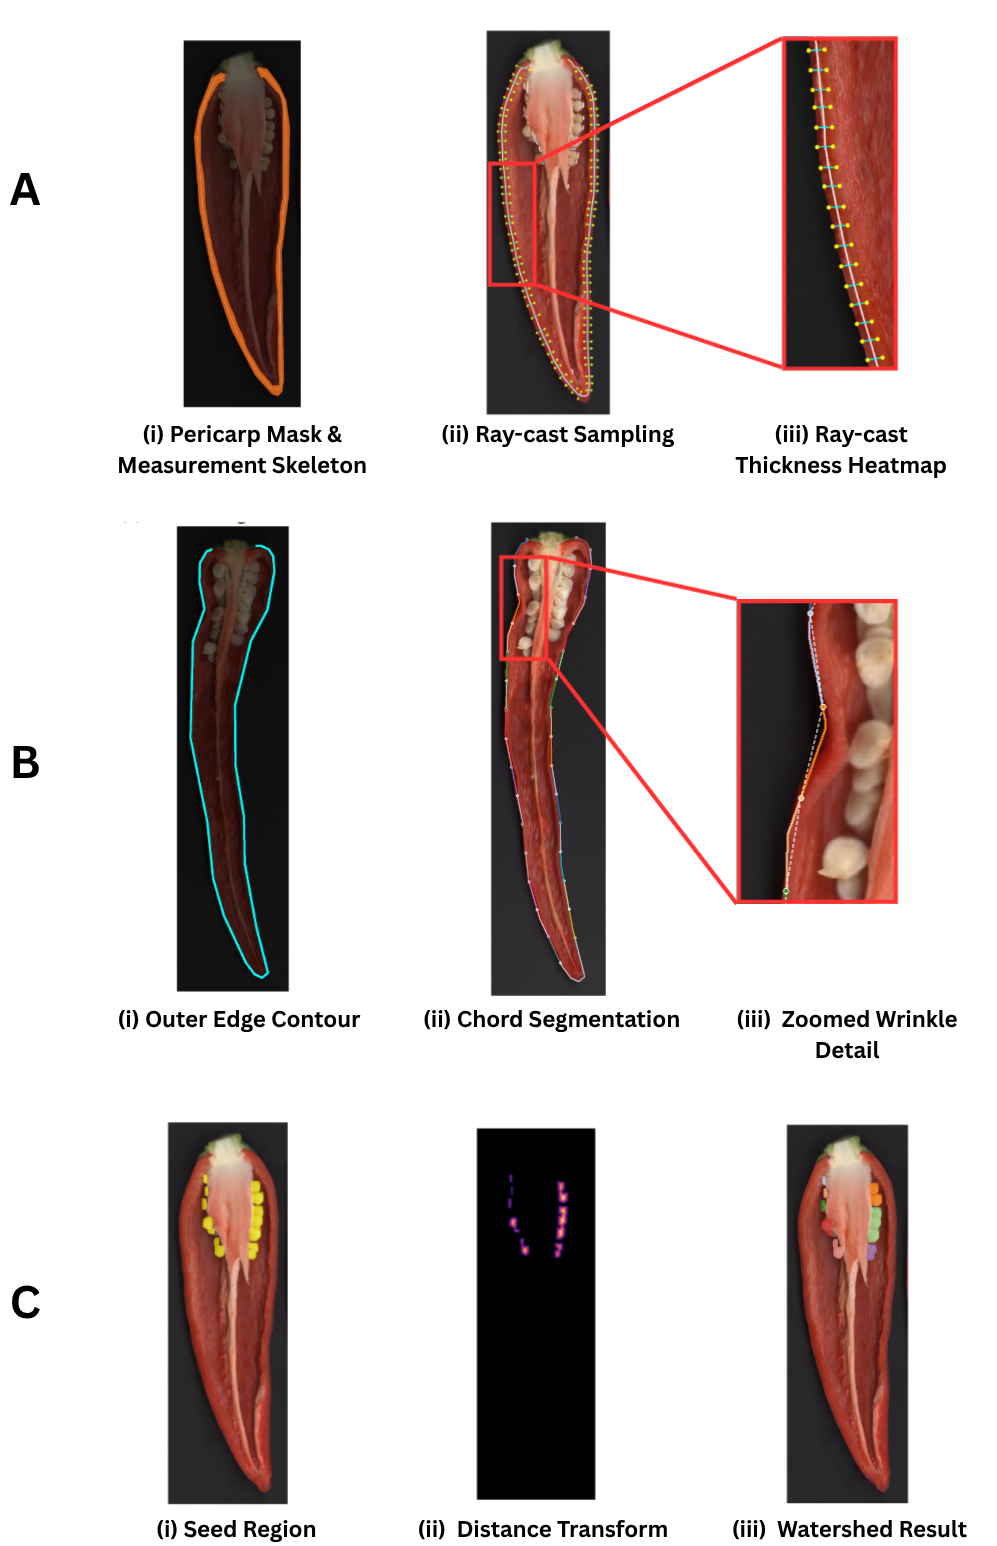
\includegraphics[width=0.9\linewidth,height=0.48\textheight,keepaspectratio]{images/fig_2.png}
\caption[\textbf{Extraction of mesocarp thickness, fruit-body contour irregularity, and seed count.} (A) Mesocarp thickness is estimated at sampled skeleton locations by selecting the shortest valid line through each location that intersects the inner and outer mesocarp boundaries. (B) Contour irregularity is summarized by the mean of one minus the chord-to-arc length ratio on the external contour of the fruit-body mask, using a 5 mm chord threshold. (C) The earlier watershed seed-separation workflow is shown for comparison; the present $SA$ and $SC$ measurements use YOLO seed instance masks.]{\textbf{Extraction of mesocarp thickness, fruit-body contour irregularity, and seed count.} (A) Mesocarp thickness is estimated at sampled skeleton locations by selecting the shortest valid line through each location that intersects the inner and outer mesocarp boundaries. (B) Contour irregularity is summarized by the mean of one minus the chord-to-arc length ratio on the external contour of the fruit-body mask, using a 5 mm chord threshold. (C) The earlier watershed seed-separation workflow is shown for comparison; the present $SA$ and $SC$ measurements use YOLO seed instance masks.\par\smallskip{\color{viColor}\textbf{VI.} \textbf{Trích xuất độ dày trung quả bì, mức độ không đều của contour thân quả và số hạt.} (A) Độ dày trung quả bì được ước lượng tại các vị trí lấy mẫu trên khung xương bằng cách chọn đoạn thẳng hợp lệ ngắn nhất đi qua từng vị trí và giao với đường biên trong và ngoài của trung quả bì. (B) Mức độ không đều của contour được tính bằng trung bình của một trừ tỷ số chiều dài dây cung trên chiều dài cung của contour ngoài mask thân quả, với ngưỡng dây cung 5 mm. (C) Quy trình tách hạt bằng watershed trước đây được minh họa để đối chiếu; phép đo $SA$ và $SC$ hiện tại sử dụng các mask instance hạt của YOLO.}}
\label{fig:method_thickness_wrinkle_seed}
\end{figure}

\section{Results / {\color{viColor} Kết quả}}

\subsection{Instance Segmentation Performance / {\color{viColor} Hiệu năng phân đoạn thực thể}}

\begin{table*}[htbp]
\centering
\caption[Comparison of YOLO instance-segmentation models on the accession-held-out test set at an input resolution of \texttt{imgsz=960}. Metrics are macro-averaged over the four reported anatomical classes: seed, outer, placenta, and endocarp.]{Comparison of YOLO instance-segmentation models on the accession-held-out test set at an input resolution of \texttt{imgsz=960}. Metrics are macro-averaged over the four reported anatomical classes: seed, outer, placenta, and endocarp.\par\smallskip{\color{viColor}\textbf{VI.} So sánh các mô hình phân đoạn thực thể YOLO trên tập kiểm thử tách biệt theo mẫu nguồn gen ở độ phân giải đầu vào \texttt{imgsz=960}. Các chỉ số được lấy trung bình macro trên bốn lớp giải phẫu được báo cáo: seed, outer, placenta và endocarp.}}
\label{tab:model_comparison}
\begin{tabular}{lcccc}
\hline
\tablevi{Model}{Mô hình} & \tablevi{Precision (\%)}{Độ chuẩn xác} & \tablevi{Recall (\%)}{Độ bao phủ} & mAP@0.5 (\%) & mAP@0.5:0.95 (\%) \\
\hline
YOLOv8s-seg & 88.78 & 79.75 & 85.01 & 45.22 \\
YOLOv8m-seg & 86.53 & 82.77 & 85.74 & 46.47 \\
YOLO11s-seg & 85.74 & 82.63 & 84.05 & 45.15 \\
YOLO11m-seg & 84.31 & 84.18 & 84.99 & 45.88 \\
YOLO26s-seg & 83.14 & 78.79 & 80.44 & 42.84 \\
YOLO26m-seg & 86.36 & 77.80 & 81.26 & 43.33 \\
\hline
\end{tabular}
\end{table*}

Table~\ref{tab:model_comparison} reports mask-based Precision, Recall, mAP@0.5, and mAP@0.5:0.95, macro-averaged over the four anatomical classes, for six candidate architectures evaluated on the accession-held-out test set. YOLOv8m-seg achieved the highest mask mAP@0.5 (85.74\%) among the six evaluated models. Its mask mAP@0.5:0.95 was 46.47\%. YOLOv8m-seg was selected as the final backbone based on its highest mAP@0.5 and moderate computational cost. Per-class results are reported in Table~\ref{tab:per_class}.

\begin{viet}
Bảng~\ref{tab:model_comparison} báo cáo Precision, Recall, mAP@0.5 và mAP@0.5:0.95 dựa trên mask, lấy trung bình macro trên bốn lớp giải phẫu, của sáu kiến trúc ứng viên được đánh giá trên tập kiểm thử tách biệt theo mẫu nguồn gen. YOLOv8m-seg đạt mask mAP@0.5 cao nhất (85.74\%) trong sáu mô hình được đánh giá. Mask mAP@0.5:0.95 của mô hình là 46.47\%. YOLOv8m-seg được chọn làm mô hình nền tảng cuối cùng dựa trên mAP@0.5 cao nhất và chi phí tính toán vừa phải. Kết quả theo từng lớp được báo cáo trong Bảng~\ref{tab:per_class}.
\end{viet}


\begin{table}[htbp]
\centering
\caption[Per-class mask-segmentation performance of the selected YOLOv8m-seg model at \texttt{imgsz=960} on the accession-held-out test set. The composite placenta--pedicel class is denoted PCP in the runtime implementation and ``placenta'' in the evaluation files.]{Per-class mask-segmentation performance of the selected YOLOv8m-seg model at \texttt{imgsz=960} on the accession-held-out test set. The composite placenta--pedicel class is denoted PCP in the runtime implementation and ``placenta'' in the evaluation files.\par\smallskip{\color{viColor}\textbf{VI.} Hiệu năng phân đoạn mask theo từng lớp của mô hình YOLOv8m-seg được chọn tại \texttt{imgsz=960} trên tập kiểm thử tách biệt theo mẫu nguồn gen. Lớp kết hợp nhau quả--cuống quả được ký hiệu PCP trong chương trình khi chạy và ``placenta'' trong các tệp đánh giá.}}
\label{tab:per_class}
\resizebox{\linewidth}{!}{\begin{tabular}{lccccc}
\hline
\tablevi{Class}{Lớp} & \tablevi{Precision (\%)}{Độ chuẩn xác} & \tablevi{Recall (\%)}{Độ bao phủ} & F1-score (\%) & mAP@0.5 (\%) & mAP@0.5:0.95 (\%) \\
\hline
\tablevi{Seed}{Hạt} & 94.48 & 92.62 & 93.54 & 95.37 & 53.81 \\
\tablevi{Outer}{Vùng ngoài mặt cắt} & 83.15 & 70.89 & 76.53 & 85.85 & 51.18 \\
\tablevi{PCP (placenta--pedicel)}{Nhau quả--cuống quả} & 90.99 & 89.64 & 90.31 & 93.83 & 62.59 \\
\tablevi{Endocarp}{Nội quả bì} & 77.51 & 77.95 & 77.73 & 67.93 & 18.32 \\
\hline
\end{tabular}}
\end{table}

\subsection{Phenotypic Trait Extraction Results / {\color{viColor} Kết quả trích xuất đặc trưng kiểu hình}}

\begin{table*}[htbp]
\centering
\footnotesize
\caption[Descriptive statistics of selected phenotypic traits calculated from 264 individual chili-fruit crops. Each crop contributes one fruit-level observation; the 367 images reported for the full dataset refer to original multi-fruit images. CV denotes the coefficient of variation (SD/mean $\times100$).]{Descriptive statistics of selected phenotypic traits calculated from 264 individual chili-fruit crops. Each crop contributes one fruit-level observation; the 367 images reported for the full dataset refer to original multi-fruit images. CV denotes the coefficient of variation (SD/mean $\times100$).\par\smallskip{\color{viColor}\textbf{VI.} Thống kê mô tả các đặc trưng kiểu hình được chọn, tính từ 264 crop quả ớt riêng lẻ. Mỗi crop đóng góp một quan sát ở cấp quả; 367 ảnh được báo cáo cho toàn bộ bộ dữ liệu là các ảnh gốc chứa nhiều quả. CV là hệ số biến thiên (SD/trung bình $\times100$).}}
\label{tab:descriptive_stats}
\resizebox{\textwidth}{!}{
\begin{tabular}{llcccc}
\hline
\tablevi{\textbf{Domain}}{Nhóm} & \tablevi{\textbf{Trait}}{Đặc trưng} & \tablevi{\textbf{Unit}}{Đơn vị} & \tablevi{\textbf{Mean $\pm$ SD}}{Trung bình ± độ lệch chuẩn} & \tablevi{\textbf{Min -- Max}}{Nhỏ nhất -- lớn nhất} & \tablevi{\textbf{CV (\%)}}{Hệ số biến thiên} \\
\hline
\multirow{8}{*}{\tablevi{Size \& Geometric}{Kích thước \& hình học}}
 & \tablevi{Fruit Length ($FL$)}{Chiều dài quả} & mm & 105.00 $\pm$ 38.10 & 26.06 -- 221.64 & 36.3 \\
 & \tablevi{Mean Fruit Width ($FW_{mean}$)}{Chiều rộng quả trung bình} & mm & 23.05 $\pm$ 16.30 & 7.17 -- 76.23 & 70.7 \\
 & \tablevi{Minimum Fruit Width ($FW_{min}$)}{Chiều rộng quả nhỏ nhất} & mm & 14.41 $\pm$ 11.16 & 3.79 -- 60.10 & 77.5 \\
 & \tablevi{Maximum Fruit Width ($FW_{max}$)}{Chiều rộng quả lớn nhất} & mm & 28.06 $\pm$ 19.16 & 9.34 -- 85.09 & 68.3 \\
 & \tablevi{Fruit Area ($FA$)}{Diện tích quả} & mm$^2$ & 2320.47 $\pm$ 2018.59 & 281.47 -- 11151.25 & 87.0 \\
 & \tablevi{Mesocarp Area ($MA$)}{Diện tích trung quả bì} & mm$^2$ & 565.03 $\pm$ 522.52 & 68.93 -- 2666.87 & 92.5 \\
 & \tablevi{Mean Mesocarp Thickness ($MT_{mean}$)}{Độ dày trung quả bì trung bình} & mm & 2.50 $\pm$ 1.93 & 0.77 -- 8.51 & 77.1 \\
 & \tablevi{Maximum Mesocarp Thickness ($MT_{max}$)}{Độ dày trung quả bì lớn nhất} & mm & 4.66 $\pm$ 3.70 & 1.15 -- 15.80 & 79.3 \\
\hline
\multirow{4}{*}{\tablevi{Internal Anatomical \& Seed}{Giải phẫu bên trong \& hạt}}
 & \tablevi{Placenta Area ($PA$)}{Diện tích nhau quả} & mm$^2$ & 420.01 $\pm$ 338.79 & 52.16 -- 1861.93 & 80.7 \\
 & \tablevi{Mesocarp Area Fraction ($MAF$)}{Tỷ phần diện tích trung quả bì} & -- & 0.25 $\pm$ 0.05 & 0.15 -- 0.42 & 20.1 \\
 & \tablevi{Seed Count ($SC$)}{Số hạt} & \tablevi{seed}{hạt} & 11.94 $\pm$ 8.11 & 0.00 -- 40.00 & 67.9 \\
 & \tablevi{Seed-to-Cavity Area Ratio ($SCR$)}{Tỷ số diện tích hạt trên khoang quả} & -- & 0.11 $\pm$ 0.08 & 0.00 -- 0.44 & 73.9 \\
\hline
\multirow{5}{*}{\tablevi{Shape \& Colorimetric}{Hình dạng \& màu sắc}}
 & \tablevi{Fruit Curvature Index ($FCI$)}{Chỉ số độ cong quả} & -- & 0.99 $\pm$ 0.02 & 0.89 -- 1.00 & 1.8 \\
 & \tablevi{Fruit Asymmetry Index ($FAI$)}{Chỉ số bất đối xứng của quả} & -- & 0.05 $\pm$ 0.03 & 0.01 -- 0.21 & 67.1 \\
 & \tablevi{Mesocarp Wrinkle Index ($MWI$)}{Chỉ số độ nhăn trung quả bì} & -- & 0.15 $\pm$ 0.18 & 0.04 -- 1.23 & 119.2 \\
 & \tablevi{Redness}{Sắc đỏ} & -- & 33.51 $\pm$ 4.32 & 12.66 -- 40.53 & 12.9 \\
 & \tablevi{Color Uniformity}{Độ đồng đều màu sắc} & -- & 7.83 $\pm$ 0.82 & 5.35 -- 10.05 & 10.4 \\
\hline
\end{tabular}
}
\end{table*}


Table~\ref{tab:descriptive_stats} summarizes the selected traits for the 264 fruit cross-sections included in this analysis. Fruit Length ($FL$) had a mean of 105.00 mm and a coefficient of variation of 36.3\%. Mesocarp Area Fraction ($MAF$) had a mean of 0.25 and a coefficient of variation of 20.1\%. These descriptive statistics are calculated at the individual fruit level.

\begin{viet}
Bảng~\ref{tab:descriptive_stats} tổng hợp các đặc trưng được chọn của 264 mặt cắt quả trong phân tích này. Chiều dài quả ($FL$) có trung bình 105.00 mm và hệ số biến thiên 36.3\%. Tỷ phần diện tích trung quả bì ($MAF$) có trung bình 0.25 và hệ số biến thiên 20.1\%. Các thống kê mô tả này được tính ở cấp từng quả riêng lẻ.
\end{viet}


To assess measurement reliability in the absence of a manual reference for morphologically derived traits (e.g., $FCI$, $FAI$, and $SCR$), we quantified the proportion of total trait variance attributable to between-variety differences relative to within-variety (biological/measurement) variance using one-way ANOVA grouped by accession ($\eta^2$). Fruit Length ($FL$) and Mean Fruit Width ($FW_{\mathrm{mean}}$) exhibited a between-variety variance ratio of 98.2\% and 99.1\%, respectively, indicating that between-accession differences account for a large share of their observed variation. The advanced algorithmic traits introduced in this study likewise showed a substantial between-variety component: $FAI$ ($\eta^2=77.8\%$), $SCR$ ($\eta^2=64.4\%$), and $FCI$ ($\eta^2=54.0\%$). These results indicate substantial between-accession variation in the examined traits. However, this analysis does not distinguish measurement error from biological variation within accessions; independent reference measurements would be needed to assess measurement accuracy.

\begin{viet}
Để đánh giá độ tin cậy của phép đo khi chưa có tham chiếu thủ công cho các đặc trưng suy ra từ hình thái (ví dụ: $FCI$, $FAI$ và $SCR$), chúng tôi định lượng tỷ phần phương sai tổng của đặc trưng do khác biệt giữa các giống so với phương sai trong giống (sinh học/phép đo), bằng ANOVA một yếu tố với các nhóm theo mẫu nguồn gen ($\eta^2$). Chiều dài quả ($FL$) và chiều rộng quả trung bình ($FW_{\mathrm{mean}}$) có tỷ phần phương sai giữa các giống lần lượt là 98.2\% và 99.1\%, cho thấy khác biệt giữa các mẫu nguồn gen chiếm phần lớn biến thiên quan sát được. Các đặc trưng thuật toán nâng cao được giới thiệu trong nghiên cứu cũng có thành phần giữa các giống đáng kể: $FAI$ ($\eta^2=77.8\%$), $SCR$ ($\eta^2=64.4\%$) và $FCI$ ($\eta^2=54.0\%$). Kết quả cho thấy biến thiên đáng kể giữa các mẫu nguồn gen ở các đặc trưng được khảo sát. Tuy nhiên, phân tích này không phân biệt được sai số đo với biến thiên sinh học trong cùng mẫu nguồn gen; cần các phép đo tham chiếu độc lập để đánh giá độ chính xác đo lường.
\end{viet}


As an exploratory biological check using the 264 fruit-level observations summarized in Table~\ref{tab:descriptive_stats}, seed count and fruit-body area showed a positive Pearson correlation ($r=0.336$, $p=2.18\times10^{-8}$). After averaging both traits within each accession, the correlation was $r=0.426$ ($p=0.00494$; $n=42$ accessions). These associations describe phenotypic covariation and do not independently validate seed-count accuracy.

\begin{viet}
Trong một phép kiểm tra sinh học mang tính thăm dò sử dụng 264 quan sát ở cấp quả được tổng hợp trong Bảng~\ref{tab:descriptive_stats}, số hạt và diện tích thân quả có tương quan Pearson dương ($r=0.336$, $p=2.18\times10^{-8}$). Sau khi lấy trung bình cả hai đặc trưng trong từng mẫu nguồn gen, tương quan là $r=0.426$ ($p=0.00494$; $n=42$ mẫu nguồn gen). Các mối liên hệ này mô tả sự đồng biến thiên kiểu hình và không phải bằng chứng kiểm chứng độc lập cho độ chính xác đếm hạt.
\end{viet}


\begin{figure}[htbp]
\centering
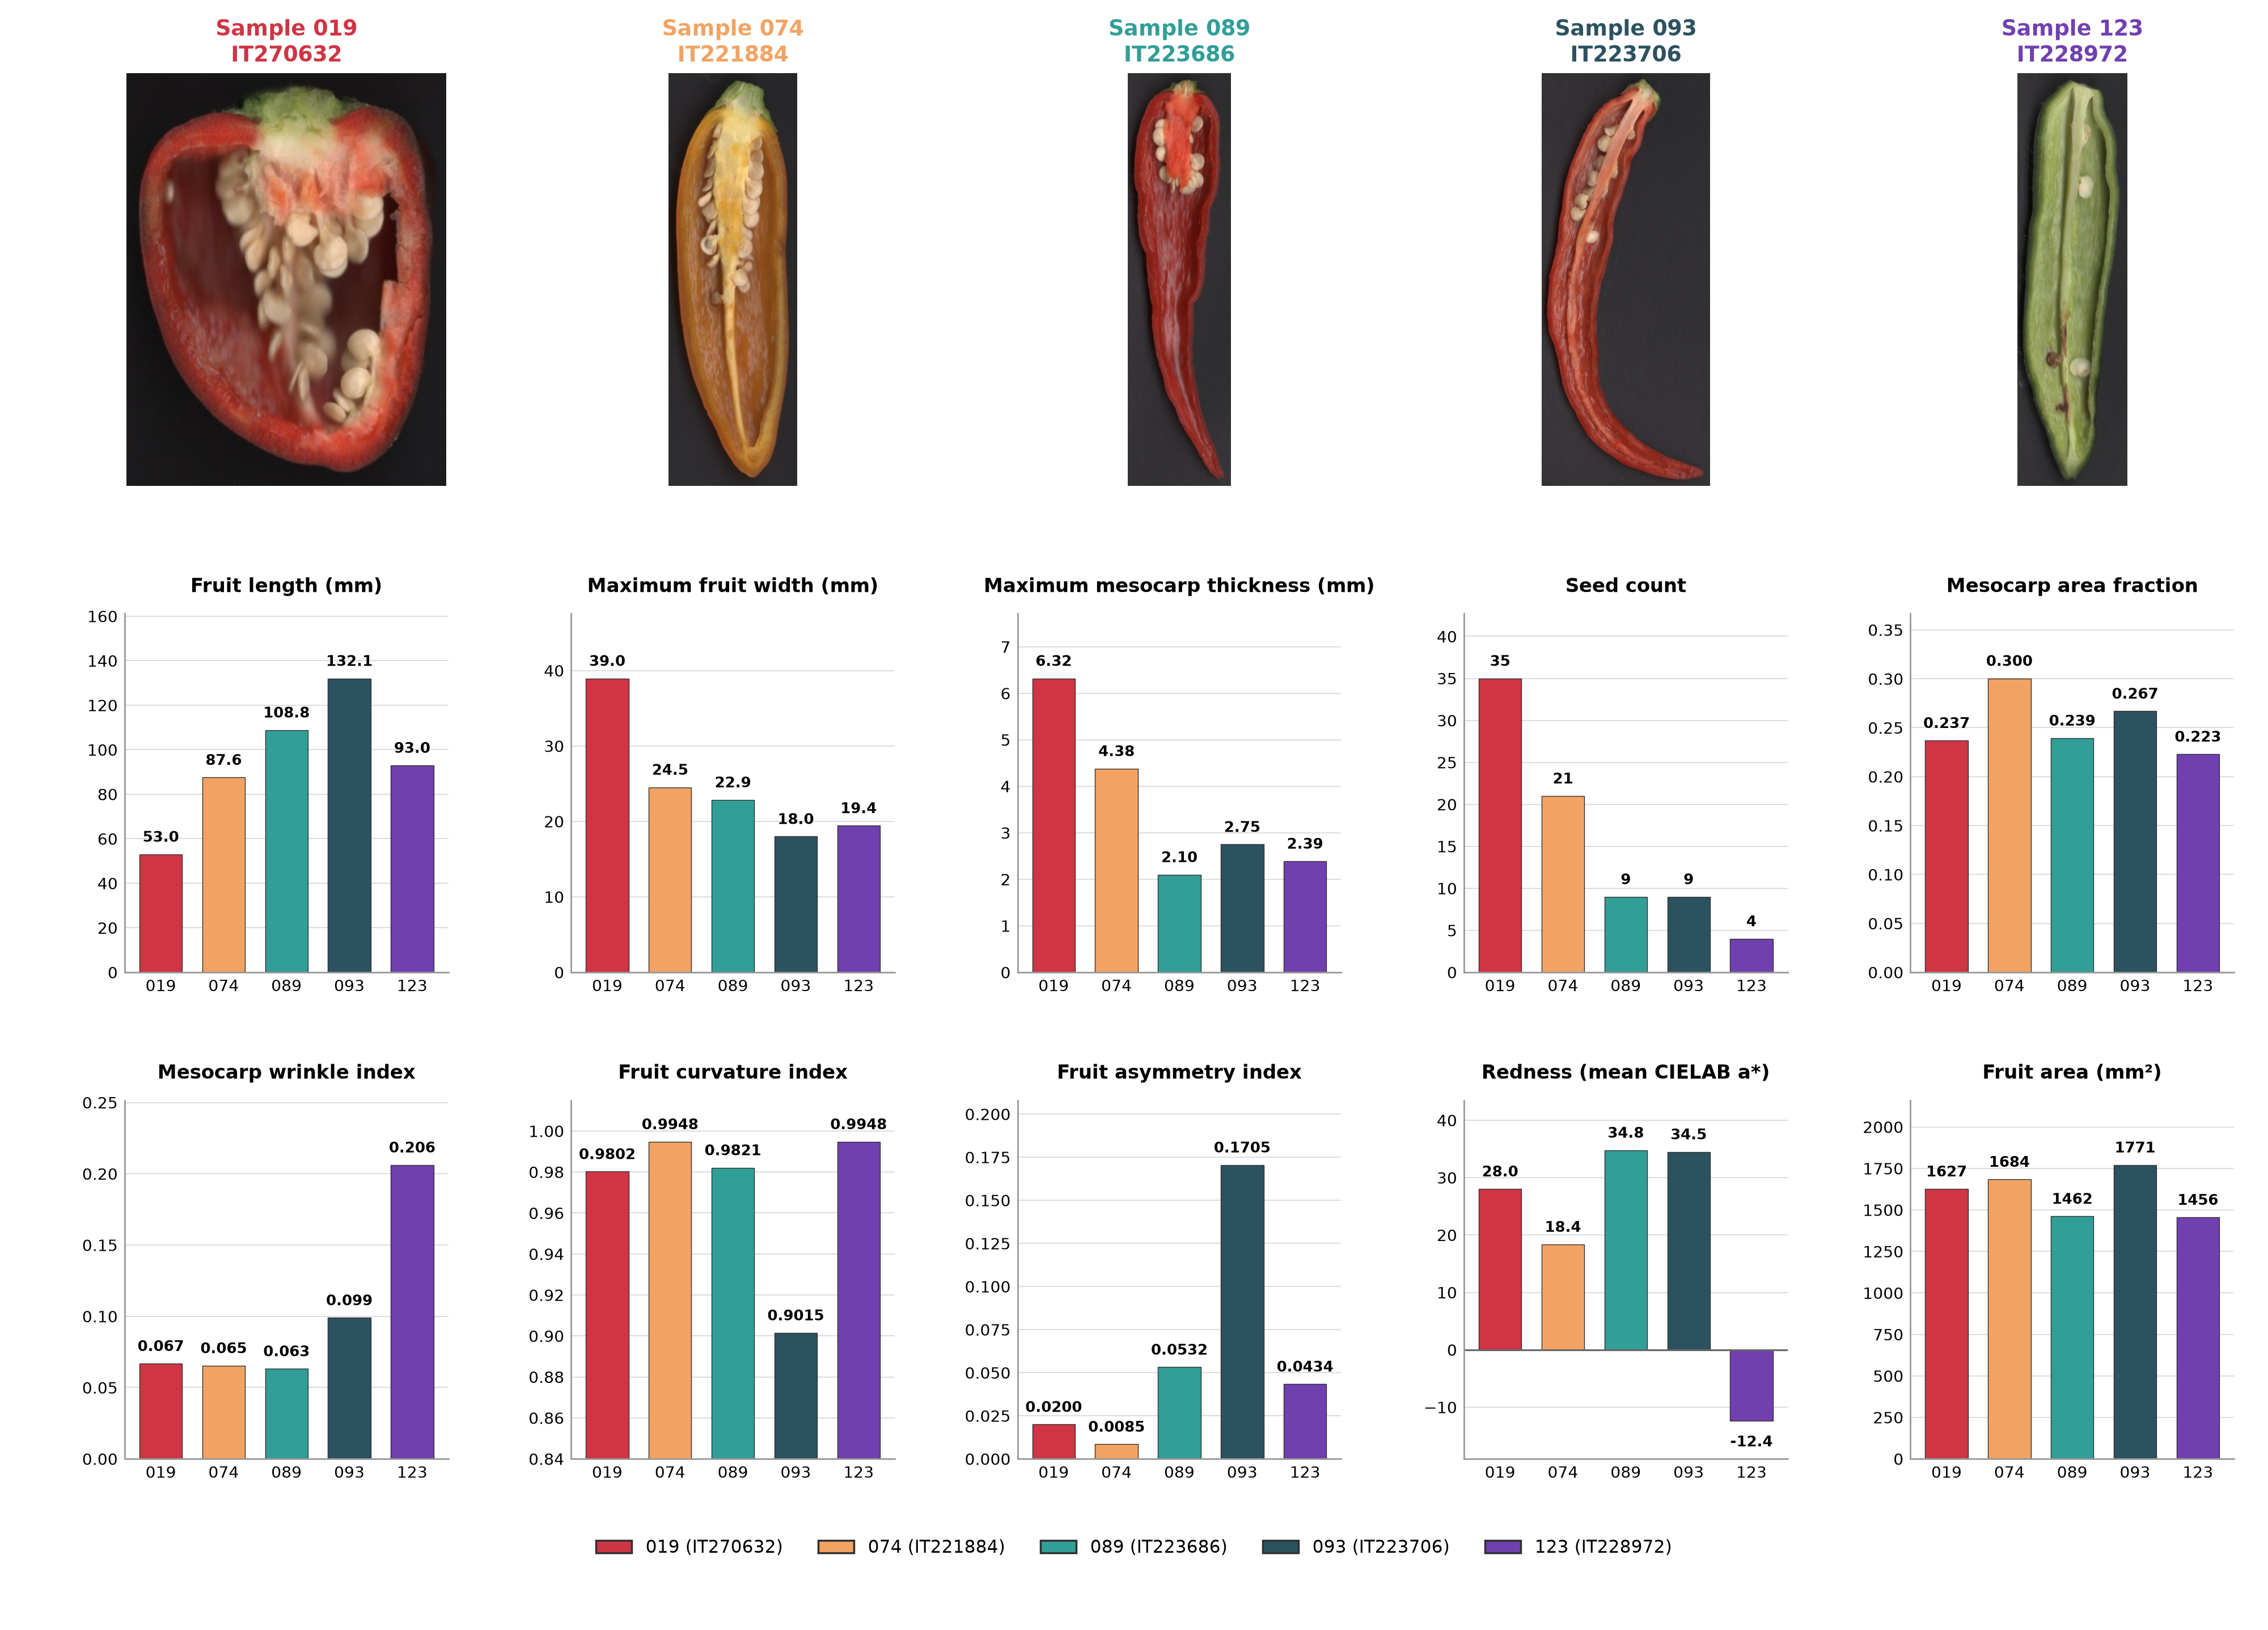
\includegraphics[width=0.9\linewidth,height=0.48\textheight,keepaspectratio]{images/Sample.png}
\caption[\textbf{Automated phenotyping of five example longitudinally sectioned chili fruits.} The images show the leftmost fruit from images 019 (IT270632), 074 (IT221884), 089 (IT223686), 093 (IT223706), and 123 (IT228972); each image is cropped and scaled independently for display. From left to right, the bar-chart panels report Fruit Length ($FL$), Maximum Fruit Width ($FW_{\max}$), Maximum Mesocarp Thickness ($MT_{\max}$), Seed Count ($SC$), Mesocarp Area Fraction ($MAF$), Mesocarp Wrinkle Index ($MWI$), Fruit Curvature Index ($FCI$), Fruit Asymmetry Index ($FAI$), mean CIELAB $a^*$ redness, and Fruit Area ($FA$). Linear measurements are in mm and fruit area is in mm$^2$; the indices are dimensionless. Values above the bars are rounded for display.]{\textbf{Automated phenotyping of five example longitudinally sectioned chili fruits.} The images show the leftmost fruit from images 019 (IT270632), 074 (IT221884), 089 (IT223686), 093 (IT223706), and 123 (IT228972); each image is cropped and scaled independently for display. From left to right, the bar-chart panels report Fruit Length ($FL$), Maximum Fruit Width ($FW_{\max}$), Maximum Mesocarp Thickness ($MT_{\max}$), Seed Count ($SC$), Mesocarp Area Fraction ($MAF$), Mesocarp Wrinkle Index ($MWI$), Fruit Curvature Index ($FCI$), Fruit Asymmetry Index ($FAI$), mean CIELAB $a^*$ redness, and Fruit Area ($FA$). Linear measurements are in mm and fruit area is in mm$^2$; the indices are dimensionless. Values above the bars are rounded for display.\par\smallskip{\color{viColor}\textbf{VI.} \textbf{Tự động phân tích kiểu hình của năm quả ớt cắt dọc minh họa.} Các ảnh thể hiện quả ngoài cùng bên trái từ các ảnh gốc 019 (IT270632), 074 (IT221884), 089 (IT223686), 093 (IT223706) và 123 (IT228972); mỗi ảnh được cắt và điều chỉnh tỷ lệ độc lập để hiển thị. Từ trái sang phải, các biểu đồ cột báo cáo chiều dài quả ($FL$), chiều rộng quả lớn nhất ($FW_{\max}$), độ dày trung quả bì lớn nhất ($MT_{\max}$), số hạt ($SC$), tỷ phần diện tích trung quả bì ($MAF$), chỉ số độ nhăn trung quả bì ($MWI$), chỉ số độ cong quả ($FCI$), chỉ số bất đối xứng của quả ($FAI$), sắc đỏ CIELAB $a^*$ trung bình và diện tích quả ($FA$). Các phép đo độ dài có đơn vị mm và diện tích quả có đơn vị mm$^2$; các chỉ số không có thứ nguyên. Giá trị phía trên các cột được làm tròn để hiển thị.}}
\label{fig:sample}
\end{figure}


\section{Discussion / {\color{viColor} Thảo luận}}

This study presents an integrated, pixel-level deep learning framework for the comprehensive automated phenotyping of chili peppers. By employing instance segmentation rather than relying solely on bounding-box representations, the proposed approach resolves the boundary ambiguities inherent in overlapping and soft biological tissues \cite{robotic,instance}. The resulting phenotypic profiles confirm that both external and internal traits, including fruit area, placenta area, seed count, mesocarp thickness, and curvature, vary continuously across cultivars, enabling fine-grained morphological characterization beyond generic shape classification.

\begin{viet}
Nghiên cứu này trình bày một hệ thống học sâu tích hợp ở cấp pixel để tự động phân tích toàn diện kiểu hình quả ớt. Bằng cách sử dụng phân đoạn thực thể thay vì chỉ dựa vào biểu diễn hộp giới hạn, phương pháp đề xuất giải quyết sự mơ hồ của đường biên vốn có ở các mô sinh học mềm và chồng lấp \cite{robotic,instance}. Hồ sơ kiểu hình thu được xác nhận rằng cả các đặc trưng bên ngoài và bên trong, gồm diện tích quả, diện tích nhau quả, số hạt, độ dày trung quả bì và độ cong, đều biến thiên liên tục giữa các giống; nhờ đó có thể mô tả hình thái chi tiết vượt ra ngoài việc phân loại hình dạng chung.
\end{viet}


\subsection*{Model selection rationale / {\color{viColor} Cơ sở lựa chọn mô hình}}
Table~\ref{tab:model_comparison} compares six instance-segmentation architectures using the same accession-held-out test set, input resolution, four reported classes, and evaluation protocol. YOLOv8m-seg achieved the highest macro-averaged mask mAP@0.5 (85.74\%) among the six evaluated models. Its mask mAP@0.5:0.95 was 46.47\%, indicating strong performance under the stricter overlap criterion. YOLOv8m-seg was therefore selected as the final segmentation backbone based on the combined consideration of segmentation quality and computational cost.

\begin{viet}
Bảng~\ref{tab:model_comparison} so sánh sáu kiến trúc phân đoạn thực thể với cùng tập kiểm thử tách biệt theo mẫu nguồn gen, độ phân giải đầu vào, bốn lớp được báo cáo và quy trình đánh giá. YOLOv8m-seg đạt mask mAP@0.5 trung bình macro cao nhất (85.74\%) trong sáu mô hình. Mask mAP@0.5:0.95 của mô hình là 46.47\%, cho thấy hiệu năng cao dưới tiêu chí chồng lấp nghiêm ngặt hơn. Vì vậy, YOLOv8m-seg được chọn làm mô hình phân đoạn nền tảng cuối cùng dựa trên việc cân nhắc kết hợp chất lượng phân đoạn và chi phí tính toán.
\end{viet}


\subsection*{Methodological contributions / {\color{viColor} Đóng góp về phương pháp}}
Conventional bounding-box approaches inherently cannot capture the precise contours required for quantitative analysis of complex biological structures \cite{instance,gedil}. The proposed pixel-level framework delineates four annotated anatomical regions and integrates deterministic geometric algorithms, including polynomial curve fitting for length measurement and skeleton-guided boundary ray casting for mesocarp-thickness estimation.

\begin{viet}
Các cách tiếp cận hộp giới hạn thông thường về bản chất không thể biểu diễn contour chính xác cần thiết cho phân tích định lượng các cấu trúc sinh học phức tạp \cite{instance,gedil}. Hệ thống ở cấp pixel được đề xuất xác định ranh giới bốn vùng giải phẫu được gán nhãn và tích hợp các thuật toán hình học tất định, gồm khớp đường cong đa thức để đo chiều dài và chiếu tia đến đường biên có dẫn hướng bằng khung xương để ước lượng độ dày trung quả bì.
\end{viet}


A further component is the post-segmentation attempt to separate the pedicel from the composite PCP mask before calculating placenta-related traits. The procedure uses two geometric strategies in sequence; when both fail, the runtime retains the PCP mask as the estimated placenta. This conditional separation reduces pedicel contamination when successful, but unresolved cases remain a potential source of bias in placenta area and related ratios.

\begin{viet}
Một thành phần khác là bước thử tách cuống khỏi mask PCP kết hợp sau phân đoạn, trước khi tính các đặc trưng liên quan đến nhau quả. Quy trình sử dụng tuần tự hai chiến lược hình học; khi cả hai thất bại, chương trình giữ mask PCP làm nhau quả ước lượng. Việc tách có điều kiện này giảm sự lẫn cuống khi thành công, nhưng các trường hợp chưa tách được vẫn là nguồn sai lệch tiềm tàng của diện tích nhau quả và các tỷ số liên quan.
\end{viet}


\subsection*{Limitations / {\color{viColor} Hạn chế}}
Despite these contributions, several limitations should be acknowledged. First, the outer class remained comparatively challenging, with an F1-score of 76.53\%, while endocarp achieved an mAP@0.5:0.95 of 18.32\% under the stricter overlap criterion. Second, precisely delineating individual seeds under dense occlusion remains challenging. The previously evaluated adaptive Watershed method reported bulk seed count agreement ($R^2=0.989$); this result does not establish the accuracy of the YOLO instance counts used here. Resolving the exact boundaries of highly overlapping seed instances may benefit from specialized density-estimation or crowd-counting architectures \cite{x}.

\begin{viet}
Bên cạnh các đóng góp trên, nghiên cứu còn một số hạn chế. Thứ nhất, lớp outer vẫn tương đối khó phân đoạn, với F1-score 76.53\%, trong khi nội quả bì đạt mAP@0.5:0.95 là 18.32\% dưới tiêu chí chồng lấp nghiêm ngặt hơn. Thứ hai, việc xác định chính xác ranh giới từng hạt trong điều kiện che khuất dày đặc vẫn còn khó khăn. Phương pháp watershed thích nghi được đánh giá trước đây cho thấy mức độ phù hợp về tổng số hạt ($R^2=0.989$); kết quả này không xác nhận độ chính xác của số hạt đếm trực tiếp từ các instance YOLO được dùng ở đây. Việc xác định đường biên chính xác của các hạt chồng lấp mạnh có thể được cải thiện bằng các kiến trúc chuyên biệt cho ước lượng mật độ hoặc đếm đối tượng đông đúc \cite{x}.
\end{viet}


\subsection*{Future directions / {\color{viColor} Hướng phát triển}}
Future work will explore non-destructive 3D imaging modalities, such as X-ray Computed Tomography (CT), to construct volumetric phenotypic profiles without physically sectioning the fruit \cite{x, fruitseg}. Additionally, specialized boundary-refinement architectures will be investigated to improve the resolution of densely occluded seed instances, and automated marker-free calibration strategies will be pursued to enhance the robustness of physical-unit scaling.

\begin{viet}
Các nghiên cứu tiếp theo sẽ khảo sát những phương thức tạo ảnh 3D không phá hủy, như chụp cắt lớp vi tính bằng tia X (CT), để xây dựng hồ sơ kiểu hình theo thể tích mà không cần cắt quả \cite{x, fruitseg}. Ngoài ra, các kiến trúc chuyên biệt để tinh chỉnh đường biên sẽ được nghiên cứu nhằm cải thiện khả năng phân giải các thực thể hạt bị che khuất dày đặc; đồng thời, các chiến lược hiệu chuẩn tự động không cần mốc sẽ được phát triển để tăng độ vững chắc của phép quy đổi sang đơn vị vật lý.
\end{viet}



\section{Conclusion / {\color{viColor} Kết luận}}
This study successfully establishes an automated, high-throughput phenotyping pipeline for chili pepper cross-sections, driven by the YOLOv8m instance segmentation architecture. By clearly defining four anatomical segmentation classes and establishing a robust optical preprocessing protocol, the proposed system effectively overcomes traditional agricultural imaging challenges, including indistinct tissue boundaries and severe seed occlusions. The strong performance of this deep learning framework provides a solid foundation for the precise digitization of internal microstructures at pixel-level resolution.

\begin{viet}
Nghiên cứu đã xây dựng thành công một quy trình tự động phân tích kiểu hình mặt cắt quả ớt với thông lượng cao, dựa trên kiến trúc phân đoạn thực thể YOLOv8m. Bằng cách định nghĩa rõ bốn lớp phân đoạn giải phẫu và thiết lập quy trình tiền xử lý quang học vững chắc, hệ thống đề xuất khắc phục hiệu quả các khó khăn truyền thống của tạo ảnh nông nghiệp, bao gồm đường biên mô không rõ và hiện tượng che khuất hạt nghiêm trọng. Hiệu năng cao của hệ thống học sâu này tạo nền tảng vững chắc cho việc số hóa chính xác các vi cấu trúc bên trong ở độ phân giải cấp pixel.
\end{viet}


Beyond conventional two-dimensional geometric measurements, the primary contribution of this work lies in the automated extraction of a comprehensive profile comprising many quantitative traits. Specifically, the system successfully quantifies advanced metrics, including the Fruit Curvature Index ($FCI$), Mesocarp Wrinkle Index ($MWI$), Seed-to-Cavity Area Ratio ($SCR$), and Fruit Asymmetry Index ($FAI$). Compared to time-consuming, error-prone, and subjective manual measurements, this approach enables the construction of a reliable, scalable, and standardized digital database, thereby significantly enhancing the reproducibility of morphological assessments in agriculture \cite{gedil}.

\begin{viet}
Vượt ra ngoài các phép đo hình học hai chiều thông thường, đóng góp chính của công trình là tự động trích xuất một hồ sơ toàn diện gồm nhiều đặc trưng định lượng. Cụ thể, hệ thống định lượng thành công các chỉ số nâng cao, gồm chỉ số độ cong quả ($FCI$), chỉ số độ nhăn trung quả bì ($MWI$), tỷ số diện tích hạt trên khoang quả ($SCR$) và chỉ số bất đối xứng của quả ($FAI$). So với các phép đo thủ công tốn thời gian, dễ sai sót và mang tính chủ quan, phương pháp này cho phép xây dựng cơ sở dữ liệu số đáng tin cậy, có khả năng mở rộng và được chuẩn hóa, qua đó cải thiện đáng kể khả năng tái lập các đánh giá hình thái trong nông nghiệp \cite{gedil}.
\end{viet}


From a practical perspective, this framework functions as a precise, automated measurement tool with strong potential for integration into industrial agricultural sorting and quality control pipelines. Future deployment efforts will prioritize adapting the model for lightweight edge-computing devices (e.g., NVIDIA Jetson) to enable real-time, in-field phenotypic screening. Ultimately, this work contributes to the advancement of data-driven precision agriculture by supporting more informed decision-making in crop breeding, genetic analysis, and agricultural research \cite{next}.

\begin{viet}
Về ứng dụng thực tế, hệ thống này là công cụ đo tự động chính xác, có tiềm năng lớn để tích hợp vào các quy trình phân loại và kiểm soát chất lượng nông sản ở quy mô công nghiệp. Các hoạt động triển khai tiếp theo sẽ ưu tiên điều chỉnh mô hình cho các thiết bị điện toán biên gọn nhẹ (ví dụ: NVIDIA Jetson), nhằm cho phép sàng lọc kiểu hình theo thời gian thực ngay tại đồng ruộng. Công trình góp phần thúc đẩy nông nghiệp chính xác dựa trên dữ liệu bằng cách hỗ trợ đưa ra quyết định có cơ sở hơn trong chọn tạo giống cây trồng, phân tích di truyền và nghiên cứu nông nghiệp \cite{next}.
\end{viet}



\section*{Declaration of generative AI and AI-assisted technologies in the writing process / {\color{viColor} Tuyên bố về AI tạo sinh và các công nghệ hỗ trợ bởi AI trong quá trình viết}}
%% TODO: giữ nguyên format này nếu có dùng công cụ AI hỗ trợ viết, ví dụ:
%% "During the preparation of this work the author(s) used [TOOL NAME] in order to
%% [PURPOSE]. After using this tool/service, the author(s) reviewed and edited the
%% content as needed and take(s) full responsibility for the content of the publication."
%% Nếu không dùng công cụ AI nào, có thể bỏ hẳn mục này.

\section*{Funding / {\color{viColor} Tài trợ}}
%% TODO: điền nguồn tài trợ thật (ẩn danh hoặc để trống cho tới bản camera-ready
%% nếu portal yêu cầu blind review tuyệt đối).

\section*{CRediT authorship contribution statement / {\color{viColor} Tuyên bố đóng góp của tác giả theo CRediT}}
%% TODO: điền vai trò từng tác giả theo chuẩn CRediT, ví dụ:
%% Author 1: Writing (original draft), Software, Methodology, Data curation.
%% Author 2: Writing (review \& editing), Funding acquisition, Conceptualization.
%% Để ẩn danh trong giai đoạn review, có thể dùng "Author A", "Author B"... thay tên thật.

\section*{Declaration of competing interest / {\color{viColor} Tuyên bố về xung đột lợi ích}}
The authors declare that the research was conducted in the absence of any commercial or financial relationships that could be construed as a potential conflict of interest.

\begin{viet}
Các tác giả tuyên bố rằng nghiên cứu được thực hiện khi không có bất kỳ mối quan hệ thương mại hoặc tài chính nào có thể được xem là xung đột lợi ích tiềm ẩn.
\end{viet}


\section*{Data availability / {\color{viColor} Khả năng truy cập dữ liệu}}
%% TODO: nêu rõ chính sách chia sẻ dữ liệu, ví dụ "Data will be made available on request."
%% hoặc link repository công khai nếu có.


%% TÀI LIỆU THAM KHẢO


\input{references_original.bbl}

\end{document}
